% LaTeX Template for Project Report, Version 2.0
% (Abstracted from a Major Project Report at CSED, NIT Calicut but can be
% modified easily to use for other reports also.)
%
% Released under Creative Commons Attribution license (CC-BY)
% Info: http://creativecommons.org/licenses/by/3.0/
%
% Created by: Kartik Singhal
% BTech CSE Batch of 2009-13
% NIT Calicut
% Contact Info: kartiksinghal@gmail.com
%
% It is advisable to learn the basics of LaTeX before using this template.
% A good resource to start with is http://en.wikibooks.org/wiki/LaTeX/
%
% All template fields are marked with a pair of angular brackets e.g. <title here>
% except for the ones defining citation names in ref.tex.
%
% Empty space after chapter/section/subsection titles can be used to insert text.
%
% Just compile this file using pdflatex after making all required changes.

\documentclass[12pt,a4paper]{report}
\usepackage[pdftex]{graphicx} %for embedding images
\usepackage{url} %for proper url entries
\usepackage[bookmarks, colorlinks=false, pdfborder={0 0 0}, pdftitle={<pdf title here>}, pdfauthor={<author's name here>}, pdfsubject={<subject here>}, pdfkeywords={<keywords here>}]{hyperref} %for creating links in the pdf version and other additional pdf attributes, no effect on the printed document
%\usepackage[final]{pdfpages} %for embedding another pdf, remove if not required

\usepackage{graphicx}
\usepackage{wrapfig}
\usepackage{caption}
\usepackage{subcaption}
\usepackage{todonotes}
\usepackage{amsmath}
\usepackage[]{algorithm2e}
\usepackage{listings} % Code
\usepackage{color}
\usepackage[toc,page]{appendix}

\definecolor{light-gray}{gray}{0.95}

\usepackage[T1]{fontenc} % åäö
\usepackage{lmodern} %åäö
\usepackage{pifont} %  Check marks
\usepackage{placeins}

\usepackage{xcolor}
\usepackage{pgfplots}
\usepackage{tikz}

\begin{document}
\renewcommand\bibname{References} %Renames "Bibliography" to "References" on ref page

\lstset{ %
  backgroundcolor=\color{light-gray},
  basicstyle={\scriptsize\ttfamily},
  breaklines=true, 
  tabsize=2, 
  language=C++,
  xleftmargin=0.5cm,
}

\newcommand{\class}[1]{$#1$}


\pgfplotsset{every tick label/.append style={font=\footnotesize}}

\definecolor{chunks_color}{HTML}{DFC9DC}
\definecolor{leafs_color}{HTML}{BCD6DD}
\definecolor{rendered_color}{HTML}{E6C3C3}
\definecolor{frame_render_time}{HTML}{577D47} %8E4747
\definecolor{globe_render_time}{HTML}{446A77}



%include other pages
\begin{titlepage}

\begin{center}

\textup{Master's thesis}\\[0.2in]

% Title
\Large \textbf {Design and Implementation of an Out-of-Core Globe Rendering System Using Multiple Map Services}\\[0.5in]

       \small \emph{Submitted in partial fulfillment of\\
        the requirements for the award of the degree of}
        \vspace{.2in}

       {\bf Master of Science \\in\\ Media Technology and Egineering}\\[0.5in]

% Submitted by
\normalsize Submitted by \\
\begin{table}[h]
\centering
\begin{tabular}{lr} \\
Kalle Bladin \& Erik Broberg \\ 
\end{tabular}
\end{table}

\vspace{.1in}
Examiner\\
{\textbf{Anders Ynnerman}}\\[0.2in]

Supervisor\\
{\textbf{Alexander Bock}}\\[0.2in]

\vfill

% Bottom of the page

\includegraphics[scale=0.2]{figures/logo_mt.png} \\
\Large{Department of Science and Technology}\\
\normalsize
\textsc{Link�ping University 2016}

\end{center}

\end{titlepage}

\vspace{2in}
\begin{abstract}

This thesis focuses on the design and implementation of a software system enabling out-of-core rendering of multiple map datasets mapped on virtual globes around our solar system. Challenges such as precision, accuracy, curvature and massive datasets were considered. The result is a globe visualization software using a chunked level of detail approach for rendering. The software can render texture layers of various sorts to aid in scientific visualization on top of height mapped geometry, yielding accurate visualizations rendered at interactive frame rates.

The project was conducted at the American Museum of Natural History (AMNH), New York and serves the goal of implementing a planetary visualization software to aid in public presentations and bringing space science to the public.

The work is part of the development of the software OpenSpace, which is the result of a collaboration between Link�ping University, AMNH and the National Aeronautics and Space Administration (NASA) among others.

\end{abstract} 

\cleardoublepage
%\pagebreak
\phantomsection
\addcontentsline{toc}{chapter}{Acknowledgements}
\chapter*{Acknowledgments}

We would like to give our sincerest thank you to all the people who have been involved in making this thesis work possible. Thank you Anders Ynnerman for giving us this opportunity. Thank you Carter Emmart for being an inspiring and driving force for the project and for introducing us to your passion in bringing astronomy to the general public. Thank you Vivian Trakinski for making us feel needed and useful for the project and for the museum.

Thank you Alexander Bock for your dedication in the project and the support you gave as a mentor along with Emil Axelsson during the whole project. All the people in the OpenSpace team along with our peers Michael and Sebastian, have been both inspiring, helpful and enjoyable to work and share the experiance with.

We would like to thank all the people we have met during our time at the American Museum of Natural History. Kayla, Eozin, Natalia, thank you for not only being our trusted lunch mates but also great friends even outside of work.
All the rest of the people at the Science Bulletins and Rose Center Engineering, thank you for being so welcoming and helpful.

Thank you Lucian Plesea for your expert support in mapping services together with Vikram Singh for setting up the map servers we could use in our software. Thanks to Jason, Ally and David for working out a method for generating terrain models from stereo pairs of Mars imagery that we could use in our software.

Masha and the rest of the CCMC team as well as Ryan, you made our visit to NASA Goddard Space Flight Centre the best experience possible by inspiring us and giving us insight in parts of NASA's space science.

All our friends and family who came to visit us in New York, thank you for spending time with us during our leisure.

Last but not least we would like to give a huge thank you to all the new friends we met during our stay in the United States. You made the experience even more enjoyable.

\newpage


\pagenumbering{roman} %numbering before main content starts
\tableofcontents
\listoffigures

\newpage
\pagenumbering{arabic} %reset numbering to normal for the main content

%\chapter{Problem Definition}

<Problem Definition here>
 %objective changed to problem definition
\chapter{Introduction}

Scientific visualization of space research, also known as astro-visualization, becomes increasingly important for scientists to communicate their work in exploring the cosmos. 3D computer graphics has shown to be an efficient tool for bringing insights from geological and astronomical data, as spatial and temporal relations can intuitively be interpreted through 3D visualizations.

Researching and mapping out celestial bodies other than the Earth is an important part of expanding the space frontier and virtually rendering these globes using real gathered map and terrain data is a natural part of any scientifically accurate space visualization software.

Two important parts of a software for visualizing celestial bodies are terrain and atmosphere. The focus of this thesis is put on terrain rendering on globes using high fidelity geographical data such as texture maps and digital terrain models. The globe rendering feature with the research involved was implemented for the software OpenSpace. The implementation was separated enough from the main program to avoid dependencies and make the thesis independent of specific implementation details. 

\section{Background}

\subsection{OpenSpace}

OpenSpace is an open-source, interactive data visualization software with the goal of bringing astro-visualization to the broad public and serve as a platform for scientists to talk about their research. The software supports rendering across multiple screens, allowing immerse visualizations on tiled displays as well as in dome theatres \cite{openspace}.

With a real time rendering software such as OpenSpace, the human curiosity involved in exploration easily becomes obvious when the user is given the ability to freely fly around in space and near the surface of other worlds and discover places they probably never can visit in real life. This is also true for public presentations where researchers such as geologists can go into details about their knowledge in these places.

An important part of the software is to avoid the use of procedurally generated data. This is to express where the frontier of science and exploration is currently at, and how it progresses through space missions with the goal of mapping the Universe. A general globe browsing feature provides a means of communicating this progress through continuous mapping of our planets and moons.

\subsection{Globe Browsing}

The term globe browsing can be described as exploration of geospatial data on a virtual representation of a globe. The word globe is a general term used to describe nearly elliptical celestial objects such as planets, moons and asteroids.

Globe rendering with the purpose of multi scale browsing has been used for quite some time in flight simulators, map services and astro-visualization. Prerendered flight paths were visualized as early as the late 1970s by NASA's Jet Propulsion Laboratory \cite{cozzi11}. 

Google Earth \cite{googlemaps} enables browsing of the Earth within a web browser using geometries for cities of high detail. The National Oceanic and Atmospheric Administration (NOAA) provides a sophisticated sphere rendering system, ''Science On a Sphere'', with the ability to visualize a vast amount of geospatial data on spheres with a temporal dimension \cite{sos}. The project is not only a software but includes projection displays and floor plans to aid in public presentations.

There are other commercial softwares that enables larger scale visualization of the Universe with real positional data gathered through research by the National Aeronautics and Space Administration (NASA), the European Space Agency (ESA) and others. Satellite Toolkit (STK) enables this by integrating ephemeris information through the SPICE interface \cite{spice} which allows accurate placing of celestial bodies and space crafts within our solar system. Uniview from SCISS AB also enables SPICE integration with sophisticated rendering techniques and dome theatre support \cite{uniview}.

There are other significant globe browsing softwares used in dome theatres such as Microsoft's World Wide Telescope (WWT) \cite{wwt}, Evans \& Sutherland's Digistar \cite{digistar}, and Sky-Skans DigitalSky \cite{digitalsky}.

Other relevant softwares that currently do not support dome configuration rendering but none the less are very adequate in their techniques of integrating globe browsing and globe rendering include Outerra \cite{outerra} and Space Engine \cite{spaceengine}. Both focusing on merging real data with procedurally generated terrains where real data is not available.

Geographic information systems (GIS) are softwares with the purpose of gathering a wide range of geographic map data and visualizing it in various different ways. Even though most of these softwares use GIS features, many of them are not considered GIS. However, they all have the globe browsing feature in common. Technicalities in how it is implemented varies as their end target users are different.

In table \ref{table:softwares}, features relevant to globe browsing in public presentations are shown and compared between different visualization softwares that integrate globe browsing.

\begin{center}
  \begin{table}
  \caption[]{Relevant features of different globe browsing softwares}
    \label{table:softwares}
  \resizebox{\textwidth}{!}{\begin{tabular}{| r | c | c | c | c | c | c |}
    \hline
        & \textbf{Observable} & \textbf{Focus on DOME} & \textbf{Ephemeris} & \textbf{Scientific} & \textbf{Free} & \textbf{Open} \\ 
	& \textbf{Universe scale} & \textbf{configuration support} & \textbf{data integrated} & \textbf{data only} & \textbf{to use}  & \textbf{source} \\ \hline

    Google Maps &  &  &  & \ding{52} & \ding{52} & \\
    STK &  &  & \ding{52} & \ding{52} & & \\
    Uniview & \ding{52} & \ding{52} & \ding{52} & \ding{52} &  & \\
    WWT & \ding{52} & \ding{52} & \ding{52} & \ding{52} & \ding{52} & \ding{52} \\
    Digistar & \ding{52} & \ding{52} & \ding{52} & \ding{52} &  &  \\
    DigitalSky & \ding{52} & \ding{52} & \ding{52} & \ding{52} &  &  \\
    Outerra &  &  &  &  & \ding{52} & \\
    Space Engine & \ding{52}  &  & \ding{52} &  & \ding{52} & \\
    OpenSpace & Future Plan & \ding{52} & \ding{52} & \ding{52} & \ding{52} & \ding{52} \\
    \hline
  \end{tabular}}
  \end{table}
\end{center}

\section{Objectives}

The goal of this thesis is not only to provide OpenSpace with a globe browsing feature. There are some specific demands that play a significant role in the focus of this work. These features are listed below:

\begin{enumerate}
    \item Ability to retrieve map data from the most common standardized web map data interfaces: WMS, TMS, WMTS
    \item Ability to render height maps and color textures with up to 25 cm per pixel resolution
    \item Ability to layer multiple map datasets on top of each other. This makes it possible to visualize a range of scientific data about the atmosphere and the ocean on top of a textured globe
    \item Globe browsing should be done at interactive framerates: at least 60 frames per second on a modern consumer gaming graphics cards
    \item Correct positional mapping of objects rendered near the globe surface
    \item Support animation of map datasets with time resolution
\end{enumerate}

\section{Delimitations}

To focus on the important aspects of globe browsing and its purposes for public presentations, some important delimitations had to be taken into consideration.

We do not consider rendering of globes with distances to the origin greater than the radius of our solar system. Direct imaging of exoplanets is far from usable for mapping and is mainly a method for locating planets \cite{exoplanets}. Since OpenSpace does not currently aim at producing procedurally generated content, visualization of exoplanets is not the focus.

One important delimitation for the project is to limit the geometry of a globe to height mapped grids. This will make it possible to perform vertex blending on the GPU as well as simplify the implementation to a uniform method of rendering across the whole globe.

We will not focus on re-projecting maps between different georeferenced coordinate systems. Therefore the implementation must be limited to reading a specific map projection. Reprojecting maps can be considered future work to generalize the ability to read map data as well as optimizing rendering output and performance.

One goal of OpenSpace is to produce awe inspiring visual effects. The current state of the project requires the foundations to be in place and globe browsing is one of the main features that need to be implemented before real sophisticated rendering techniques can be developed. We will not consider rendering of atmospheres or water effects and we will not consider shading that requires changing of the current rendering pipeline of OpenSpace such as deferred shading.
 %literature survey included in this
\chapter{Theoretical Background}

A sophisticated globe rendering system needs to rely on some mathematical foundations. These foundations together with different theories and algorithms developed for globe rendering works as a base for the research of this thesis.

\section{Modelling Globes}

We will discuss different proposed methods used for modelling and rendering of globes. The globe can be modelled either as a sphere or an ellipsoid and there are different tessellation schemes for meshing the globe. Different map projections can also be considered and it all ties together with a choice of level of detail algorithm.

\subsection{Globes as Ellipsoids}

Planets, moons and asteroids are generally more accurately modelled as ellipsoids than as spheres. Planets are often stretched out along their equatorial axes due to their rotation which causes the centripetal force to counter some of the gravitational force acting on the mass. This effect was proven in 1687 by Isac Newton in Principia Mathematica \cite{newton87}. The rotation causes a self-gravitating fluid body in equilibrium to take the form of an oblate ellipsoid, otherwise known as a biaxial ellipsoid with one semimajor and one semiminor axis. Globes can be modeled as triaxial ellipsoids for more accuracy when it comes to smaller, more irregularly shaped objects. For example Phobos, one of Mars's two moons, is more accurately modeled as a triaxial ellipsoid with radii of $27 \times 22 \times 18$ km \cite{cozzi11}.

The World Geodetic System 1984 (WGS84) standard defined by National Geospatial-Intelligence Agency (NGA) models the Earth as a biaxial ellipsoid with a semimajor axis of 6,378,137 m and a semiminor axis of 6,356,752.3142 m \cite{cozzi11}. This is what is known as a reference ellipsoid; a mathematical description that approximates the geoid of the earth as closely as possible. The WGS84 standard is widely used for GIS and plays an important role in accurate placements of objects such as satellites or spacecrafts with position coordinates relatively close to the Earth's surface. In the WGS84 coordinate system, the x-axis points to the prime meridian, the z-axis points to the north pole and the y-axis completes the right handed coordinate system, see figure \ref{fig:wgs84}.

\begin{figure}
\centering
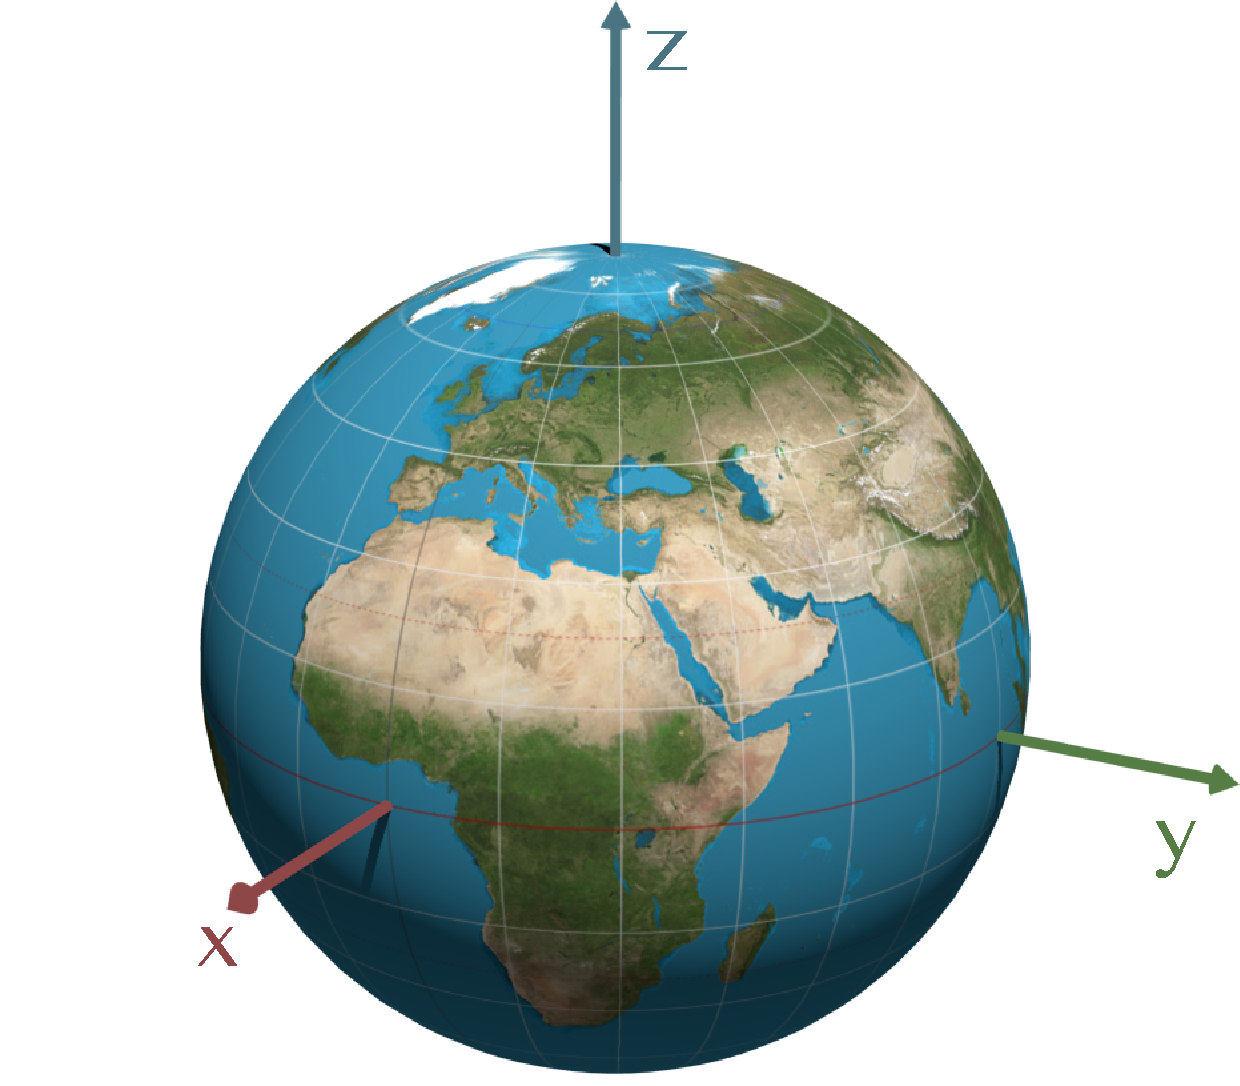
\includegraphics[scale=0.25]{figures/wgs84.pdf}
\caption{The WGS84 coordinate system and globe.}
\label{fig:wgs84}
\end{figure}

\subsection{Tesselating the Ellipsoid}

Triangle models are still the most common way of modeling renderable objects in 3D graphics softwares, even though other rendering techniques such as volumetric ray casting also is possible for terrain rendering (src).

A triangle mesh, or more generally a polygon mesh, is defined by a limited number of surface elements. This means that ellipsoids need to be approximated by some sort of tessellation or subdivision surface when modeled as a polygon mesh. There are several techniques for tessellating an ellipsoid. Some of them are covered in this section.

\subsubsection{Geographic Grid Tessellation}
\label{sec:geogrid}
Tessellating the ellipsoid using a geographic grid is a very straightforward approach. Ellipsoid vertex positions can be calculated using a transform from geographic coordinates to cartesian model space coordinates \cite[p. 25]{cozzi11}. Figure \ref{fig:tesselation_geo} shows three geographic grid tessellations of ellipsoids with constant number of latitudinal segments of 4, 8 and 16 respectively.

A common issue with geographic grids is something referred to as polar pinching. At both of the poles, segments will be pinched to one point which leads to an increasing amount of segments per area. This in turn results in oversampling in textures as well as possible visual artefacts in shading due to the very thin quads at the poles as well as possible performance penalties for highly tessellated globes.

\begin{figure}
    \centering
    \begin{subfigure}[b]{0.2\textwidth}
        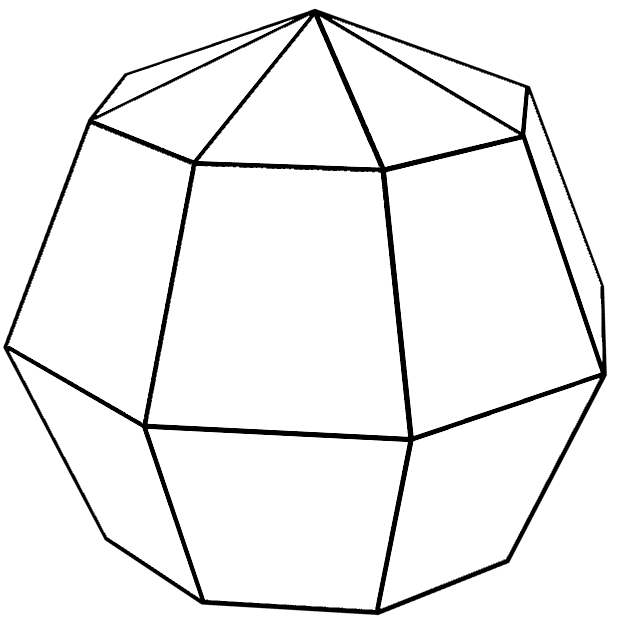
\includegraphics[width=\textwidth]{figures/tessellation/tessellation_geo1.png}
    \end{subfigure}
    ~ %add desired spacing between images, e. g. ~, \quad, \qquad, \hfill etc. 
      %(or a blank line to force the subfigure onto a new line)
    \begin{subfigure}[b]{0.2\textwidth}
        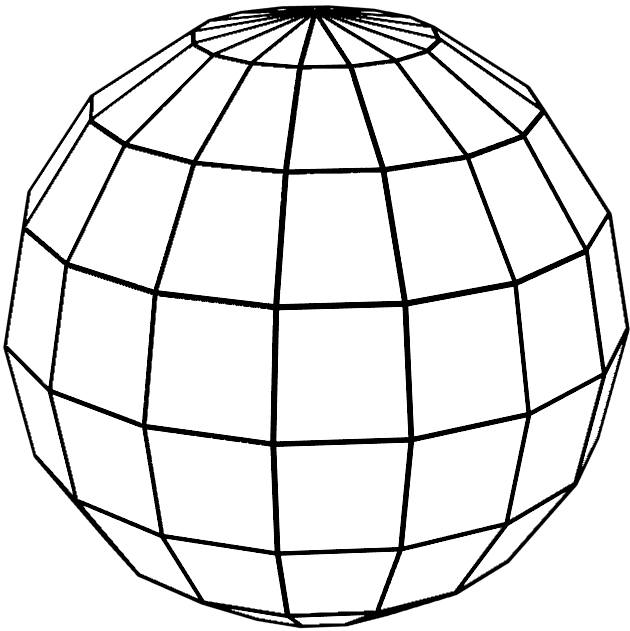
\includegraphics[width=\textwidth]{figures/tessellation/tessellation_geo2.png}
    \end{subfigure}
    ~ %add desired spacing between images, e. g. ~, \quad, \qquad, \hfill etc. 
    %(or a blank line to force the subfigure onto a new line)
    \begin{subfigure}[b]{0.2\textwidth}
        
\includegraphics[width=\textwidth]{figures/tessellation/tessellation_geo3.png}
    \end{subfigure}
    \caption{Geographic grid tesselation.}
    \label{fig:tesselation_geo}
\end{figure}

\subsubsection{Quadrilateralized Spherical Cube Tessellation}
 
Another common tessellation method for spheres which can be generalized to ellipsoids is the quadrilateralized spherical cube tessellation. The standard approach is to subdivide a cube centered in the origin and then normalize the coordinates of all vertices to map them on a sphere. There are also other more complicated schemes designed to work with specific map projections \cite{dimi15}.

To model an ellipsoid from a sphere, the vertices can be linearly transformed with a scaling in the $x$, $y$, and $z$ directions individually. Figure \ref{fig:tesselation_cube} shows a tessellated spherical cube of four different detail levels.

\begin{figure}
    \centering
    \begin{subfigure}[b]{0.2\textwidth}
        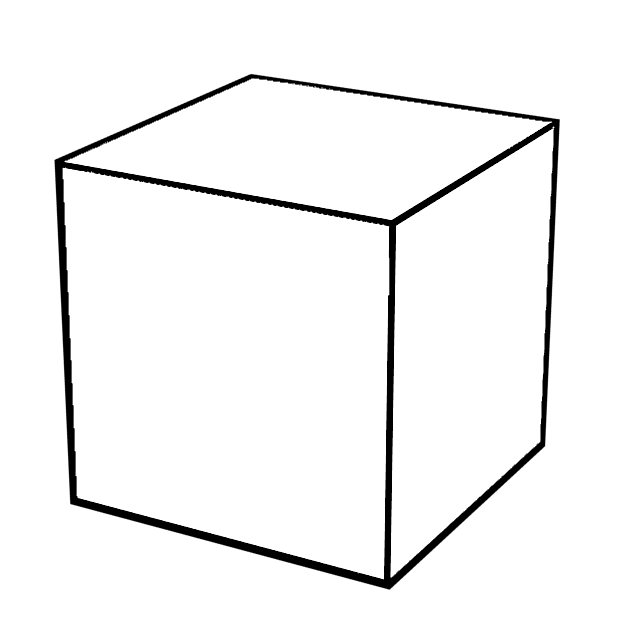
\includegraphics[width=\textwidth]{figures/tessellation/tessellation_cube1.png}
    \end{subfigure}
    ~ %add desired spacing between images, e. g. ~, \quad, \qquad, \hfill etc. 
      %(or a blank line to force the subfigure onto a new line)
    \begin{subfigure}[b]{0.2\textwidth}
        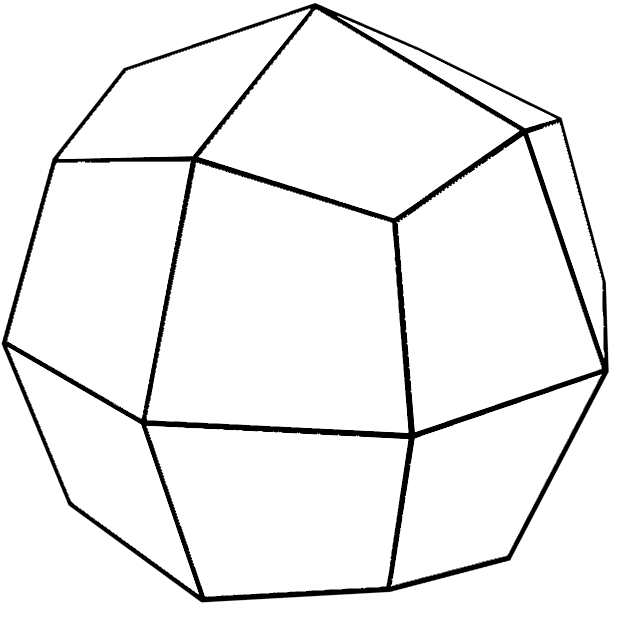
\includegraphics[width=\textwidth]{figures/tessellation/tessellation_cube2.png}
    \end{subfigure}
    ~ %add desired spacing between images, e. g. ~, \quad, \qquad, \hfill etc. 
    %(or a blank line to force the subfigure onto a new line)
    \begin{subfigure}[b]{0.2\textwidth}
        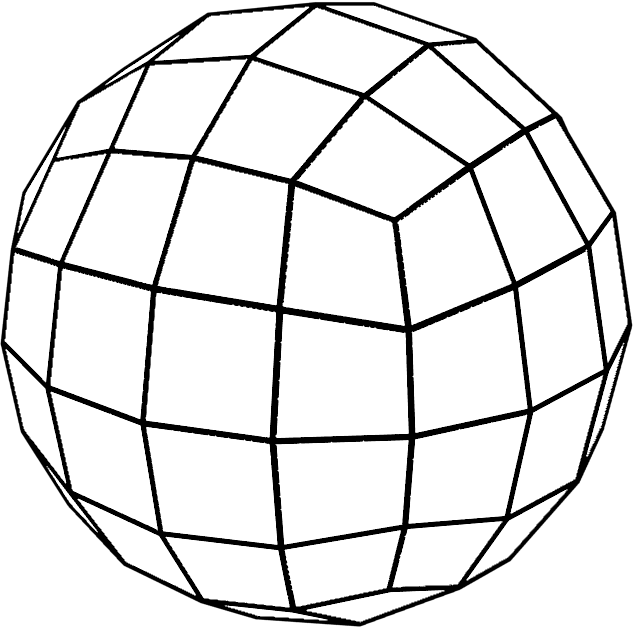
\includegraphics[width=\textwidth]{figures/tessellation/tessellation_cube3.png}
    \end{subfigure}
    ~ %add desired spacing between images, e. g. ~, \quad, \qquad, \hfill etc. 
    %(or a blank line to force the subfigure onto a new line)
    \begin{subfigure}[b]{0.2\textwidth}
        
\includegraphics[width=\textwidth]{figures/tessellation/tessellation_cube4.png}
    \end{subfigure}
    \caption{Quadrilateralized spherical cube tessellation.}
    \label{fig:tesselation_cube}
\end{figure}

\subsubsection{Hierarchical Triangular Mesh}

The hierarchical triangular mesh (HTM) is a method of modeling the sky dome as a sphere proposed by astronomers in the Sloan Digital Sky Survey \cite{htm}. Instead of uniformly dividing cube faces, an alternative option is to subdivide a normalized octahedron by, in each subdivision step, split every triangle into four new triangles, see figure \ref{fig:tesselation_htm}. An ellipsoid can be created from the sphere by normalizing the coordinates and linearly rescaling them the same way that can be done for the spherical cube tessellation.

\begin{figure}
    \centering
    \begin{subfigure}[b]{0.2\textwidth}
        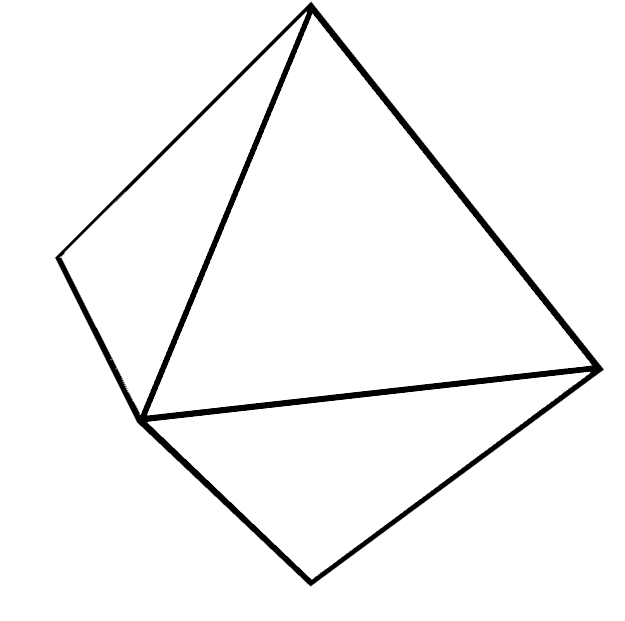
\includegraphics[width=\textwidth]{figures/tessellation/tessellation_htm1.png}
    \end{subfigure}
    ~ %add desired spacing between images, e. g. ~, \quad, \qquad, \hfill etc. 
      %(or a blank line to force the subfigure onto a new line)
    \begin{subfigure}[b]{0.2\textwidth}
        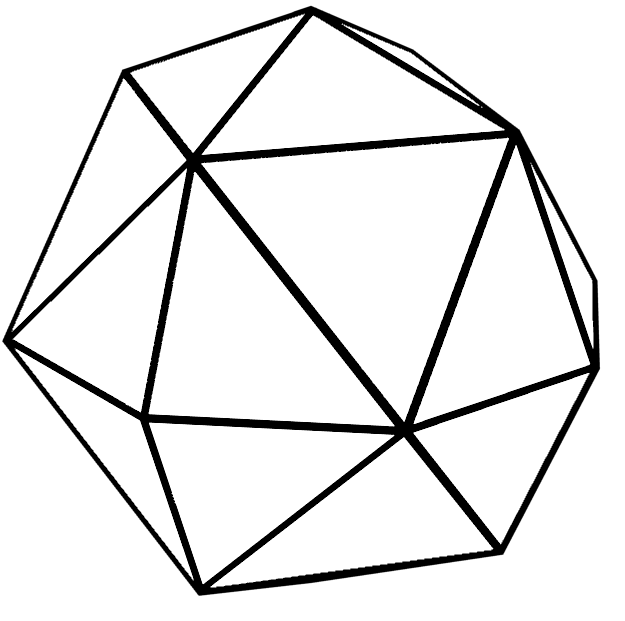
\includegraphics[width=\textwidth]{figures/tessellation/tessellation_htm2.png}
    \end{subfigure}
    ~ %add desired spacing between images, e. g. ~, \quad, \qquad, \hfill etc. 
    %(or a blank line to force the subfigure onto a new line)
    \begin{subfigure}[b]{0.2\textwidth}
        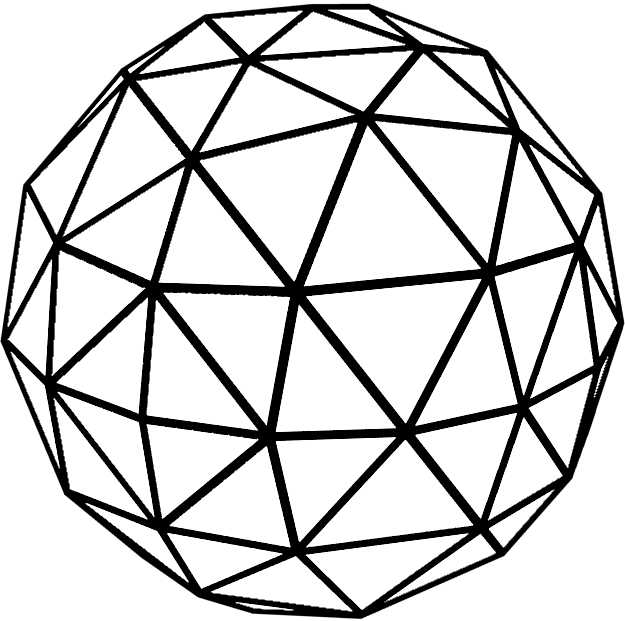
\includegraphics[width=\textwidth]{figures/tessellation/tessellation_htm3.png}
    \end{subfigure}
    ~ %add desired spacing between images, e. g. ~, \quad, \qquad, \hfill etc. 
    %(or a blank line to force the subfigure onto a new line)
    \begin{subfigure}[b]{0.2\textwidth}
        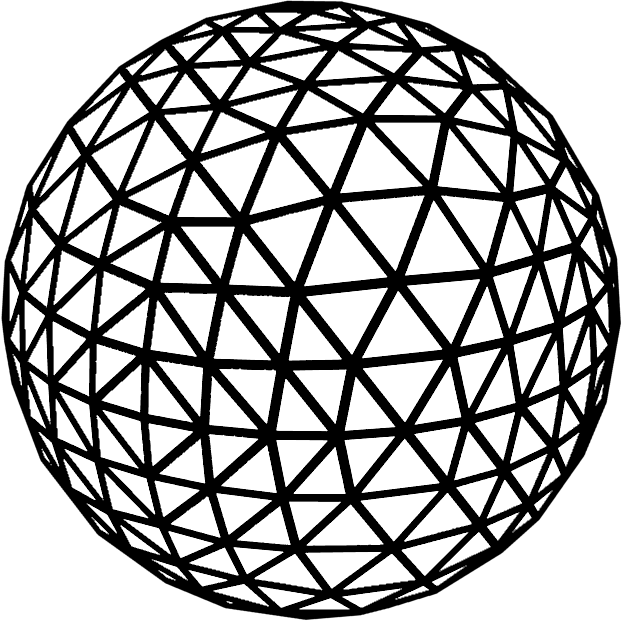
\includegraphics[width=\textwidth]{figures/tessellation/tessellation_htm4.png}
    \end{subfigure}
    \caption{Hierarchical triangular mesh tesselation.}
    \label{fig:tesselation_htm}
\end{figure}

\subsubsection{Hierarchical Equal Area IsoLatitude Pixelation}

Hierarchical Equal Area IsoLatitude Pixelation (HEALPix) is spherical tessellation scheme with corresponding map projection. The base level of the tessellation is built up of twelve quads, similar to a rhombic dodecahedron, which each can be subdivided further. The tessellation in figure \ref{fig:tesselation_healpix} shows how the vertices in the HEALPix tessellation leads to curvilinear quads.

\begin{figure}
    \centering
    \begin{subfigure}[b]{0.2\textwidth}
        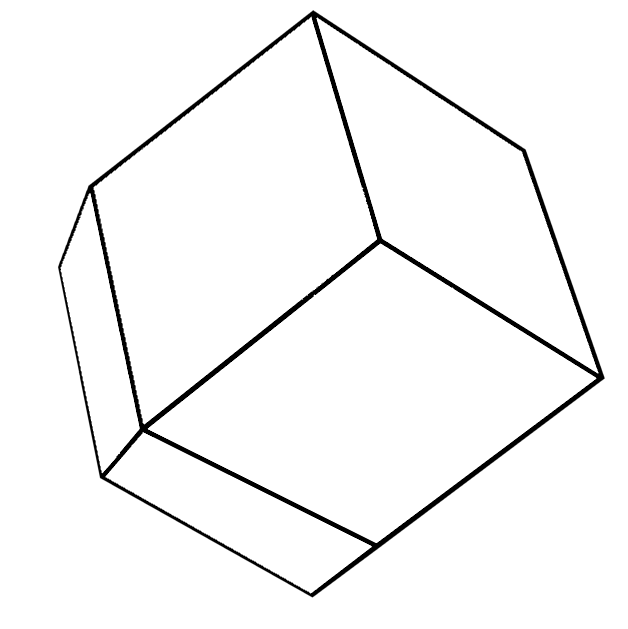
\includegraphics[width=\textwidth]{figures/tessellation/tessellation_healpix1.png}
    \end{subfigure}
    ~ %add desired spacing between images, e. g. ~, \quad, \qquad, \hfill etc. 
      %(or a blank line to force the subfigure onto a new line)
    \begin{subfigure}[b]{0.2\textwidth}
        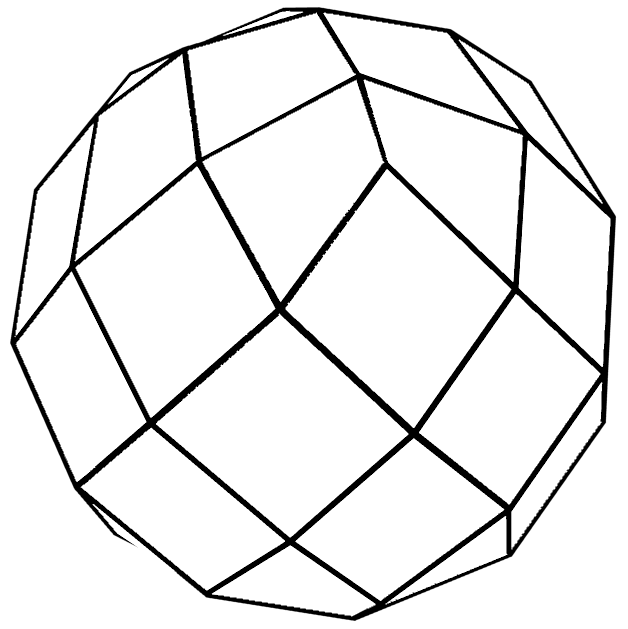
\includegraphics[width=\textwidth]{figures/tessellation/tessellation_healpix2.png}
    \end{subfigure}
    ~ %add desired spacing between images, e. g. ~, \quad, \qquad, \hfill etc. 
    %(or a blank line to force the subfigure onto a new line)
    \begin{subfigure}[b]{0.2\textwidth}
        
\includegraphics[width=\textwidth]{figures/tessellation/tessellation_healpix3.png}
    \end{subfigure}
    \caption{HEALPix tesselation.}
    \label{fig:tesselation_healpix}
\end{figure}

\subsubsection{Geographic Grid Tessellation With Polar Caps}

In their description of the ellipsoidal clipmaps method, Dimitrijevi\'{c} and Ran\v{c}i\'{c} introduces polar caps to avoid polar issues related to geographic grids \cite{dimi15}. The polar caps are simply used as a replacement of the problematic, oversampled regions around the poles. The caps can be modelled as grids projected onto the ellipsoid surface in their own georeferenced coordinate systems. One obvious issue with polar caps is the edge problem that occurs due to the fact that the caps are defined as separate meshes with vertices that do not coincide with the geographic vertices of the equatorial region, see figure caps. Dimitrijevi\'{c} and Ran\v{c}i\'{c} solves the issue by using a type of edge blending between the equatorial and polar segments \cite{dimi15}. Figure \ref{fig:tesselation_caps} shows a sphere tessellated with one equatorial region and two polar regions.

\begin{figure}
    \centering
    \begin{subfigure}[b]{0.2\textwidth}
        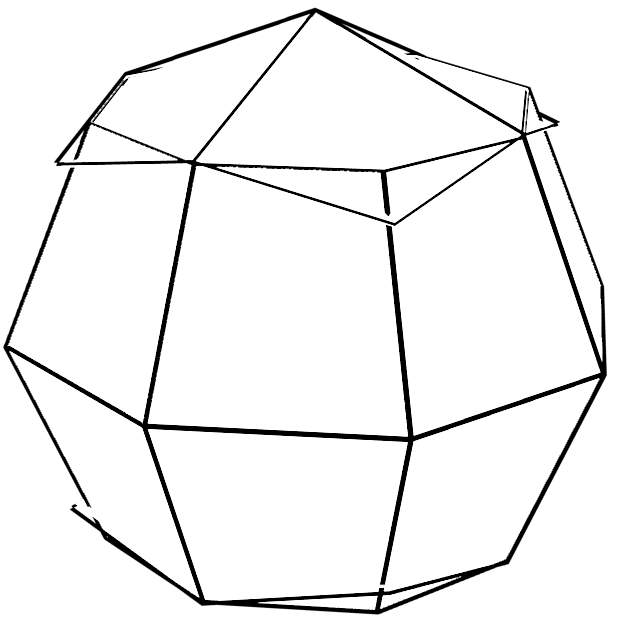
\includegraphics[width=\textwidth]{figures/tessellation/tessellation_caps_proj1.png}
    \end{subfigure}
    ~ %add desired spacing between images, e. g. ~, \quad, \qquad, \hfill etc. 
      %(or a blank line to force the subfigure onto a new line)
    \begin{subfigure}[b]{0.2\textwidth}
        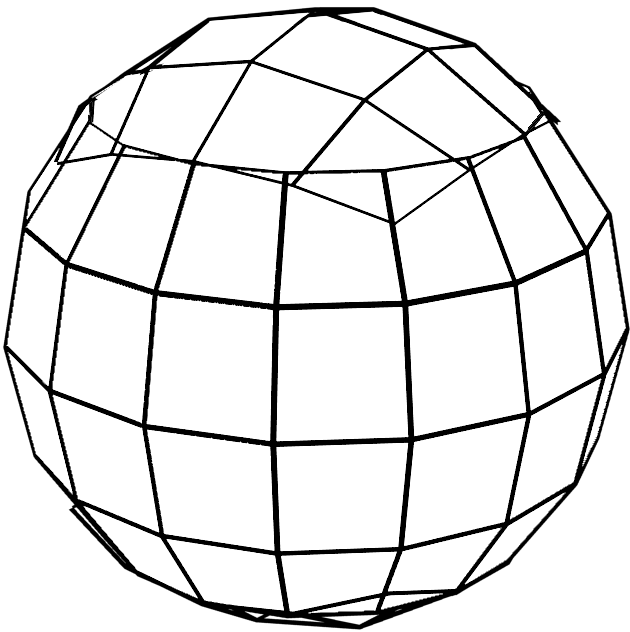
\includegraphics[width=\textwidth]{figures/tessellation/tessellation_caps_proj2.png}
    \end{subfigure}
    ~ %add desired spacing between images, e. g. ~, \quad, \qquad, \hfill etc. 
    %(or a blank line to force the subfigure onto a new line)
    \begin{subfigure}[b]{0.2\textwidth}
        
\includegraphics[width=\textwidth]{figures/tessellation/tessellation_caps_proj3.png}
    \end{subfigure}
    \caption{Geographic tessellation of an ellipsoid with polar caps.}
    \label{fig:tesselation_caps}
\end{figure}

\subsection{2D Parameterisation for Map Projections}

A map projection $P$ defines a transformation from cartesian model space coordinates to georeferenced (projected) coordinates, as in equation \ref{eq:proj}. The inverse projection $P^{-1}$ is used to find positions on the globe surface in model space given georeferenced coordinates as in equation \ref{eq:invproj}.

\begin{equation}
\label{eq:proj}
\begin{pmatrix} s  \\ t  \end{pmatrix}_{ georeferenced }=\vec { P } (x,y,z),
\end{equation}

\begin{equation}
\label{eq:invproj}
\begin{pmatrix} x \\ y \\ z \end{pmatrix}_{ modelspace }=\vec { P }^{-1} (s ,t ),
\end{equation}

Where $(x,y,z)^T$ is the cartesian coordinates of a point on the ellipsoid surface. The parameters $s$ and $t$ are georeferenced coordinates defining all positions on the globe. The georeferenced coordinates can have different definition range depending on which projection is used.

The globally positive gaussian curvature of any ellipsoid makes it impossible to unproject it on a flat 2D surface without any distortions. Different projections are used for different purposes. Equal-area projections preserve the size of a projected area as $\partial s \partial t / \partial s_0 \partial t_0 = 1$, while conformal projections preserve the shape of projected objects as $\partial s / \partial t = 1$; $s_0$ and $t_0$ are coordinates at the center of the projection with no distortion. No global projection can be both area-preserving and conformal \cite{dimi15}.

There are several possibilities for defining a coordinate transform for map projections. A common approach is to project the ellipsoid onto another shape that allows for being flattened out without distortion, such as a cube, a cylinder or a plane. These types of shapes are known as developable shapes and have zero gaussian curvature.

The choice of map projection is tied together with the choice of ellipsoid tessellation. This is because the map often needs to be tiled up when rendering. Each tile has its local texture coordinate system which need to have a simple transform from the georeferenced coordinate system for texture sampling. If the tiles can be affinely transformed to the geo referenced coordinate system, texture sampling can be done on the fly; otherwise the geo referenced coordinates need to be reprojected which may be computationally heavy or impossible for real time applications.

The European Petroleum Survey Group (EPSG) has defined several standards for map projections of the Earth. Many of these are mentioned when discussing the different projections.

\subsubsection{Geographic Projections}

Geographic projections are widely used standards for parameterization of ellipsoids. The ellipsoid is projected onto a cylinder which is then unrolled to form the 2D plane of the projected coordinates.

Geographic coordinates are defined with a latitude $\phi$ and a longitude $\theta$ and works together with geographic tessellations of ellipsoids. A common issue with geographic projections is oversampling around the poles, as mentioned in section \ref{sec:geogrid}. At the poles, all longitudes will always map onto one point and the distortion increases with the absolute value of the latitude. Figure \ref{fig:proj_equi} shows an unprojected geographic map and how it wraps around the globe.

\begin{figure}[htbp]
    \centering
    \begin{subfigure}[bt]{0.4\textwidth}
        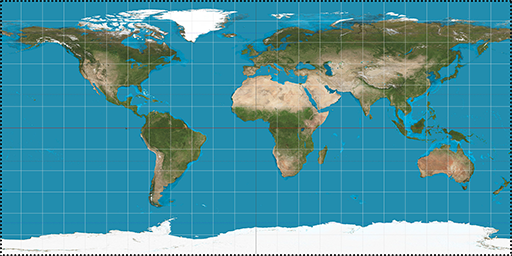
\includegraphics[width=\textwidth]{figures/developable_projected/equirectangular.png}
    \end{subfigure}
    \qquad
    \begin{subfigure}[bt]{0.15\textwidth}
        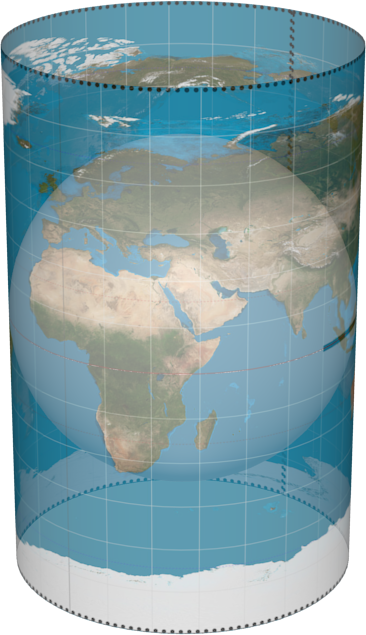
\includegraphics[width=\textwidth]{figures/map_projection/projection_geo.png}
    \end{subfigure}
    \caption{Geographic map projection.}
    \label{fig:proj_equi}
\end{figure}

\paragraph{Geocentric projection}
The simplest geographic parameterization uses geocentric coordinates. Here the latitude and longitude are defined as the angle between a vector from the origin to a point on the ellipsoid surface, and the $xy-$ and $xz-$planes respectively.

\paragraph{Geodetic projection}
The equirectangular cylindrical projection, using geodetic coordinates, is another variety of the geographic coordinate systems where the distance differential along the latitude $\partial \phi$ maps linearly to the latitude differential of the projected coordinates of the map.

Figure \ref{fig:geodetic} shows the difference between geocentric latitudes, $\phi_c$ and geodetic latitudes, $\phi_d$ for a point $\vec{p}$ on the surface of an ellipsoid. The figure also shows the difference between geocentric and geodetic surface normals, $\hat{n_c}$ and $\hat{n_d}$, respectively. 

\begin{figure}[htbp]
\centering
\begin{picture}(130,130)
    \put(0,0){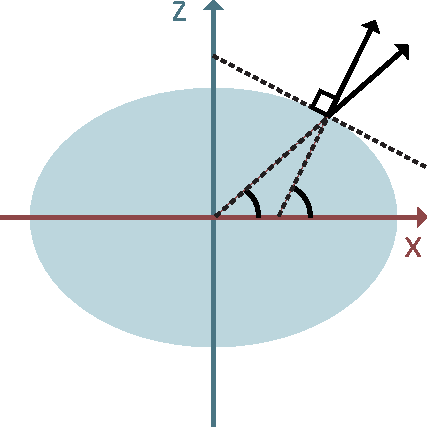
\includegraphics[width=0.35\textwidth]{figures/geodetic_geocentric.pdf}}
    \put(112,97){$\vec{p}$}
    \put(130,107){$\hat{n}_c$}
    \put(100, 130){$\hat{n}_d$}
    \put(100, 75){$\phi_d$}
    \put(82, 75){$\phi_c$}
    \label{fig:proj_equirectangular}
\end{picture}
\caption{Difference between geocentric and geodetic latitudes.}
\label{fig:geodetic}
\end{figure}

In the case of perfect spheres, geocentric and geodetic projections of any point will yield the same result.

Geodetic coordinates are among the most commonly used geo referenced coordinate systems when mapping ellipsoids to two dimensions. Latitudinal distances are preserved after the coordinate transform. This is important for a map projection standard that can be used for both spheres and for ellipsoids to avoid distortions that will appear if the map is defined for a specific ellipsoid and then projected on a slightly different one.

Equirectangular projections does not require specific ellipsoids to avoid distorsions on the mapped globe. The result of the wide usage is that many map providers choose to provide 2D maps defined in this coordinate system.

Cozzi and Ring describes the transform from geodetic coordinates in the ellipsoid class \cite[p. 25]{cozzi11}. For the Earth, the most commonly used geodetic coordinate space is defined in the EPSG:4326 standard where the WGS84 ellipsoid is used.

\subsubsection{Mercator Projection}

The mercator projection is a cylindrical projection widely used for presenting global maps in unwrapped form. The mercator projection preserves the horizontal to vertical ratio for small objects on the map. Hence, the mercator is a conformal projection in contrast to the geocentric and geodetic projections, which results in a non unit value in the ratio between the longitudinal and latitudinal differentials, see figure \ref{fig:mercator}.

\begin{figure}[htbp]
    \centering
    \begin{subfigure}[bt]{0.3\textwidth}
        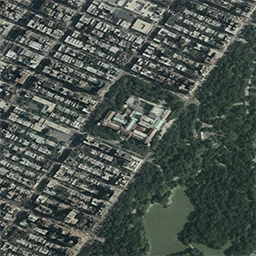
\includegraphics[width=\textwidth]{figures/central_park_equirectangular.png}
	\caption{The equirectangular projection is not conformal.}
    \end{subfigure}
    \qquad
    \begin{subfigure}[bt]{0.3\textwidth}
        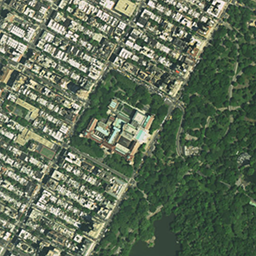
\includegraphics[width=\textwidth]{figures/central_park_mercator.png}
        \caption{The mercator projection is conformal and preserves aspect ratio.}
    \end{subfigure}
    \caption{Unwrapped equirectangular and mercator projections.}
    \label{fig:mercator}
\end{figure}

The mercator projection compensates for the longitudinal distortion by introducing a latitudinal distortion as well. Due to the polar singularities which lead to infinite latitudes at the poles when $\phi_d = \pm 90$, the domain of definition for the latitudes need to be constrained in mercator projection, see figure mercator.

\begin{figure}[htbp]
    \centering
    \begin{subfigure}[bt]{0.4\textwidth}
        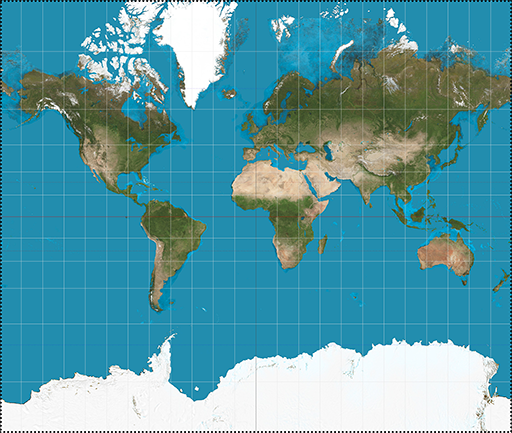
\includegraphics[width=\textwidth]{figures/developable_projected/mercator.png}
    \end{subfigure}
    \qquad
    \begin{subfigure}[bt]{0.15\textwidth}
        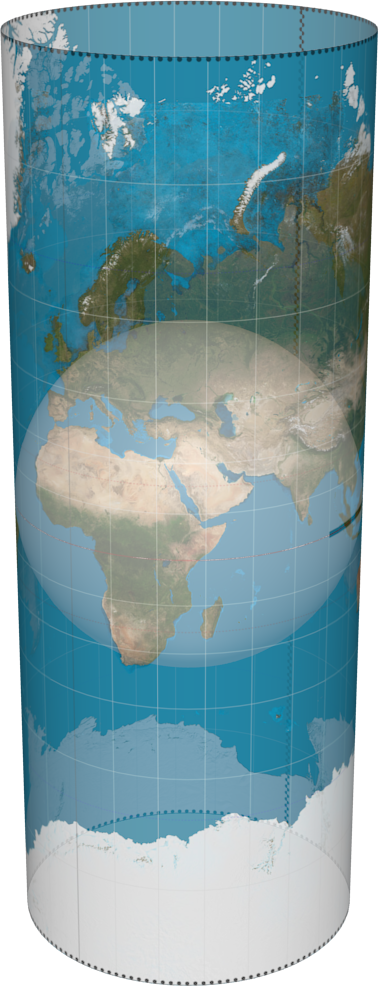
\includegraphics[width=\textwidth]{figures/map_projection/projection_mercator.png}
    \end{subfigure}
    \caption{Mercator projection.}
    \label{fig:proj_mercator}
\end{figure}

The EPSG:3857 standard for mercator projection of the Earth, also known as web mercator, constrains the domain to $\phi \in [-85.06, 85.06]$. The standard uses a different projection that does not diverge at the polar regions. Web mercator is used by most online web map applications including Google Maps, Bing Maps, OpenStreetMap, Mapquest, Esri and Mapbox \cite{battersby14}.

\subsubsection{Cube Map}

Cube maps lack the polar singularities apparent in geographic parameterizations. The parameterized coordinates are often discretized to the six sides of the cube, but they can also map directly to a global representation of an unwrapped cube, see figure \ref{fig:proj_cube}.

\begin{figure}[htbp]
    \centering
    \begin{subfigure}[bt]{0.4\textwidth}
        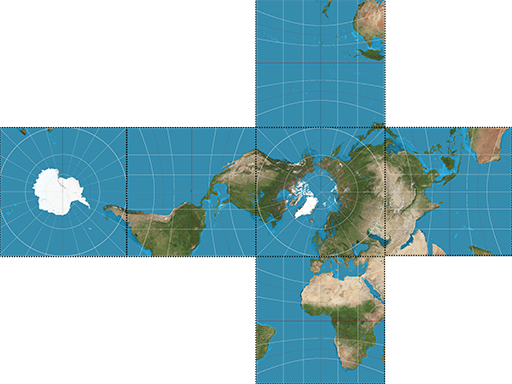
\includegraphics[width=\textwidth]{figures/developable_projected/cube_map.png}
    \end{subfigure}
    \qquad
    \begin{subfigure}[bt]{0.15\textwidth}
        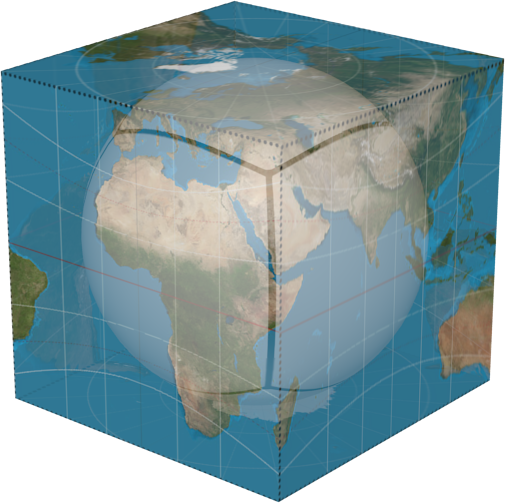
\includegraphics[width=\textwidth]{figures/map_projection/projection_cube.png}
    \end{subfigure}
    \caption{Cube map projection.}
    \label{fig:proj_cube}
\end{figure}

Due to the traditions of map projections this is not a common format used for map services so reprojection from a more common format is often required.

There are different cube map projections with different amount of area- and aspect distortions. Dimitrijevi\'{c} and Ran\v{c}i\'{c} mention and compares spherical cube, adjusted spherical cube, Outerra spherical cube and quadrilateralized spherical cube \cite{dimi15}.

\subsubsection{Tessellated Octahedral Adaptive Subdivision Transform}

The Tessellated Octahedral Adaptive Subdivision Transform (TOAST) map format used in the globe browsing of Microsoft's World Wide Telescope works together with the HTM tessellation \cite{toast}. Each triangular segment of the TOAST map maps linearly to a triangle of a sphere that is tessellated as an octahedron and subdivided to form a sphere, see figure \ref{fig:proj_toast}.

\begin{figure}[htbp]
    \centering
    \begin{subfigure}[bt]{0.3\textwidth}
        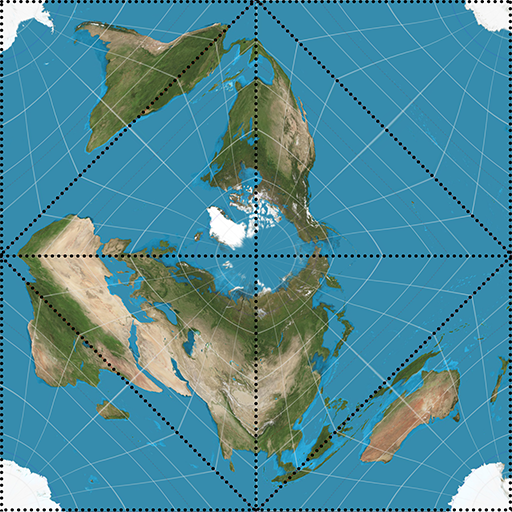
\includegraphics[width=\textwidth]{figures/developable_projected/toast.png}
    \end{subfigure}
    \qquad
    \begin{subfigure}[bt]{0.2\textwidth}
        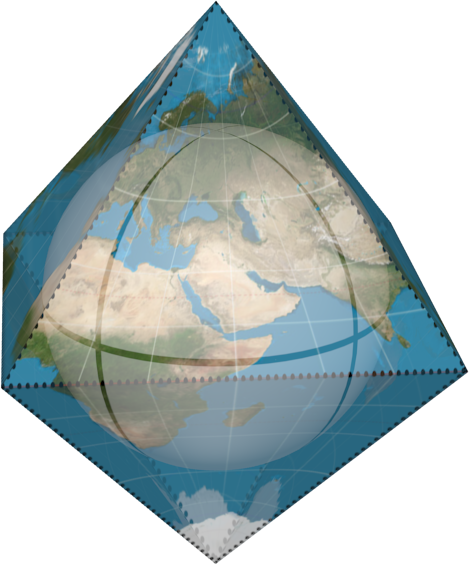
\includegraphics[width=\textwidth]{figures/map_projection/projection_toast.png}
    \end{subfigure}
    \caption{TOAST map projection.}
    \label{fig:proj_toast}
\end{figure}

The TOAST format is just as the cube maps not a very well supported format for map providers and harder to use together with some of the most common level of detail approaches due to the fact that most of them are optimized for rectangular and not triangular map tiles.

\subsubsection{Hierarchical Equal Area IsoLatitude Pixelation}

The map projection that is used for the HEALPix tessellation is equal-area as the name suggests. Figure \ref{fig:proj_healpix} shows how the map wraps onto the sphere. The positive aspect about HEALPix compared to the TOAST format is that the map is tiled into quads and not triangles which means that it is better suitable for the chunked lod \cite{cozzi11} algorithm. The map format is used by the Sloan Digital Sky Survey for mapping the cosmic microwave background radiation but is otherwise an uncommon format when it comes to map services. That means that the maps need to be reprojected from the more common formats for wider support.

\begin{figure}[htbp]
    \centering
    \begin{subfigure}[bt]{0.5\textwidth}
        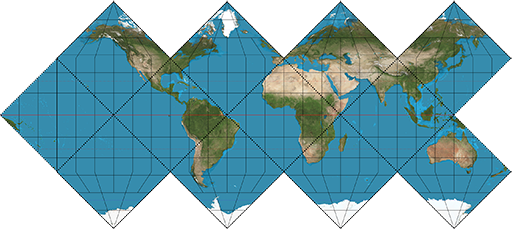
\includegraphics[width=\textwidth]{figures/developable_projected/healpix.png}
    \end{subfigure}
    \qquad
    \begin{subfigure}[bt]{0.2\textwidth}
        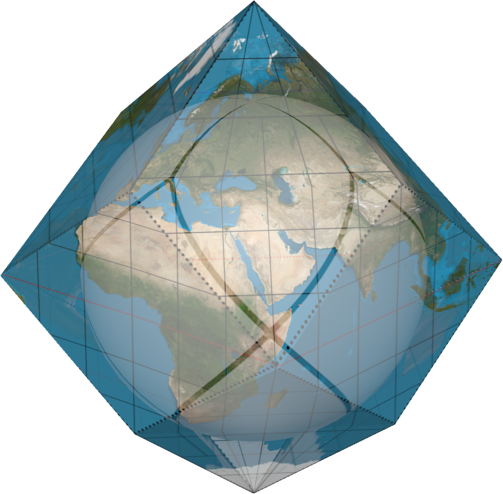
\includegraphics[width=\textwidth]{figures/map_projection/projection_healpix.png}
    \end{subfigure}
    \caption{HEALPix map projection.}
    \label{fig:proj_healpix}
\end{figure}

\subsubsection{Polar Projections}

For parameterization of limited parts of the globe, such as the isolated poles, there are different projections to consider. Most common are different types of azimuthal projections. These projections are defined by projecting all points of the map through a common intersection point and onto a flat surface. The Gnomonic projection maps all great circle segments (geodesics) to straight lines by having the common intersection point in the center of the globe.

Stereographic projections are defined when the common intersection point is positioned on the surface of the globe on the opposite side of the pole to project. Polar stereographic projections are used to parameterize the surface of the poles of the Earth. The standards EPSG:3413 and EPSG:3031 define the stereographic projections for the North Pole and the South Pole respectively.

Dimitrijevi\'{c} and Ran\v{c}i\'{c} uses another polar coordinate system to reproject from geodetic coordinates in runtime. The transformation is a rotation of 90 degrees around the global $x-$axis so that the resulting parametric coordinates of the pole are given in their own geographic space with the main meridian as equator. This projection is also known as a Cassini projection and it can be both defined for spheres as well as generalized to ellipsoids. Polar projections are shown in figure \ref{fig:proj_polar}.

\begin{figure}[htbp]
    \centering
    \begin{subfigure}[b]{0.3\textwidth}
        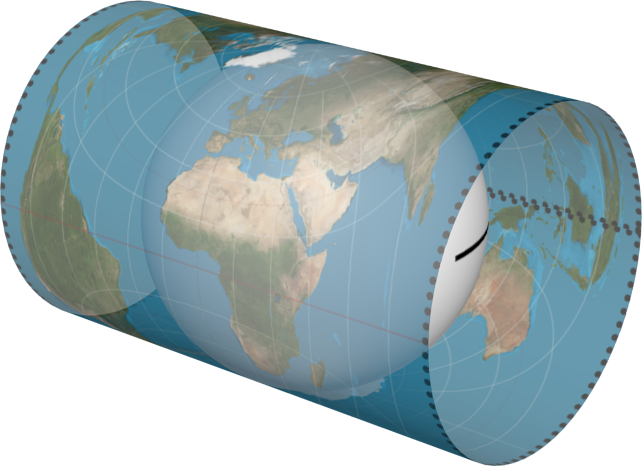
\includegraphics[width=\textwidth]{figures/map_projection/projection_cassini.png}
    	\caption{Cassini}
    \end{subfigure}
    ~
    \begin{subfigure}[b]{0.3\textwidth}
        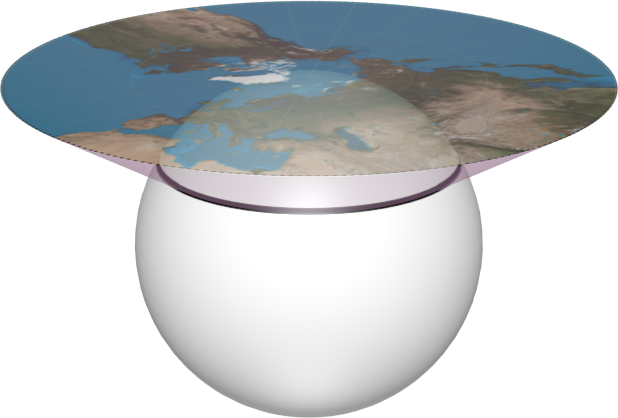
\includegraphics[width=\textwidth]{figures/map_projection/projection_gnomonic.png}
        \caption{Gnomonic}
    \end{subfigure}
    ~
    \begin{subfigure}[b]{0.3\textwidth}
        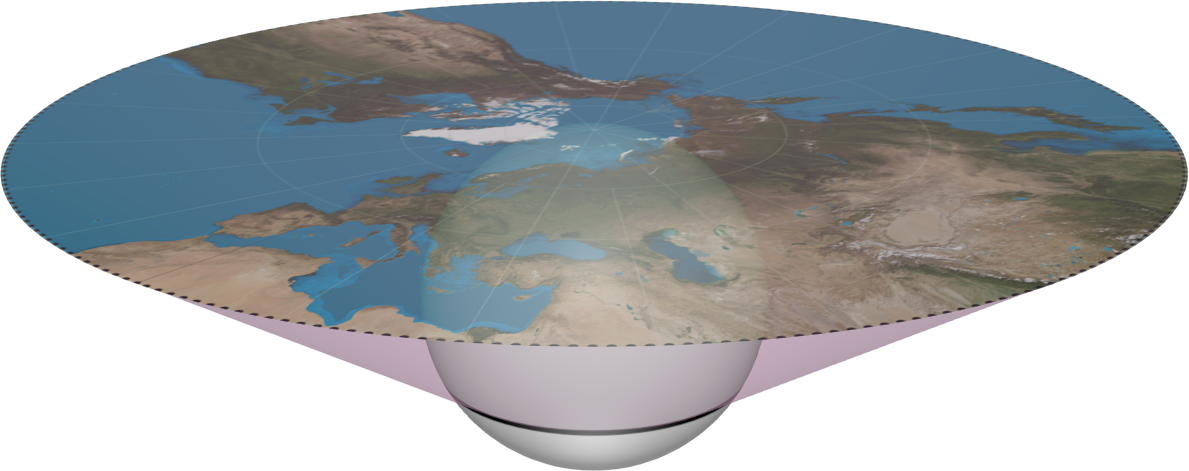
\includegraphics[width=\textwidth]{figures/map_projection/projection_stereographic.png}
    	\caption{Stereographic}
    \end{subfigure}
    \caption{Polar map projections.}
    \label{fig:proj_polar}
\end{figure}

\section{Dynamic Level of Detail}
Dynamic level of detail (LOD) is an important part in handling the extensive amount of data used in an out of core rendering software. The goal is to maximize the visual information on screen while minimizing the workload. In their book Rendering virtual 3D globes, Cozzi and Ring describes LOD rendering algorithms by three typical steps. \cite[p. 367]{cozzi11}

\begin{enumerate}
    \item Generation - Create versions at different level of detail of a model
    \item Selection - Choose a version based on some criteria or error metric (e.g., distance to object or the projected area it occupies on the screen)
    \item Switching - Transitions from one version to another in order to avoid noticing of the change in LOD known as popping artifacts.
\end{enumerate}

There are different types of LOD approaches for terrain rendering, and a suitable approach should be chosen based on characteristics of the terrain. Terrains can for example be restricted to being represented as height maps - a characteristic that can be exploited by the rendering algorithm. Cozzi and Ring describe the following three categories of LOD approaches: Discrete Level of Detail, Continuous Level of Detail and Hierarchical Level of Detail \cite[p. 368-371]{cozzi11}.

\subsection{Discrete Level of Detail}
In the Discrete Level Of Detail (DLOD) approach, multiple different representations of the terrain are created at different resolutions. DLOD is arguably the most simple LOD algorithm. It works not only for digital terrain models, but for arbitrary meshes. The set of terrain representations can either be predefined or generated using mesh simplification algorithms.

\begin{figure}[htbp]
    \centering
    \begin{subfigure}[bt]{0.9\textwidth}
        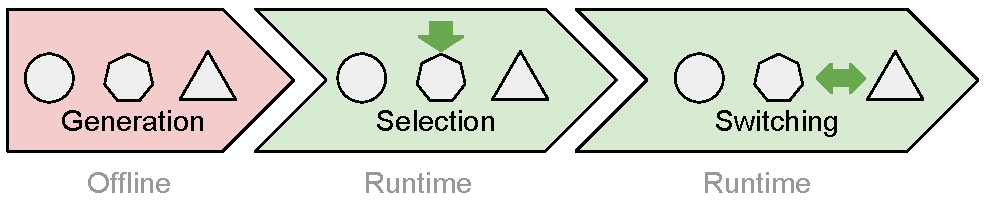
\includegraphics[width=\textwidth]{figures/lod/lod_overview.pdf}
    \end{subfigure}
    \caption{DLOD. Generate offline, select and switch at runtime.}
    \label{fig:lod}
\end{figure}

\begin{figure}
    \centering
    \begin{subfigure}[b]{0.2\textwidth}
        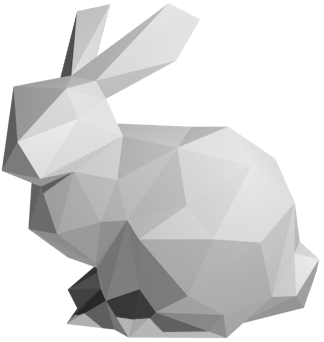
\includegraphics[width=\textwidth]{figures/lod/decimation3.png}
    \end{subfigure}
    ~ %add desired spacing between images, e. g. ~, \quad, \qquad, \hfill etc. 
      %(or a blank line to force the subfigure onto a new line)
    \begin{subfigure}[b]{0.2\textwidth}
        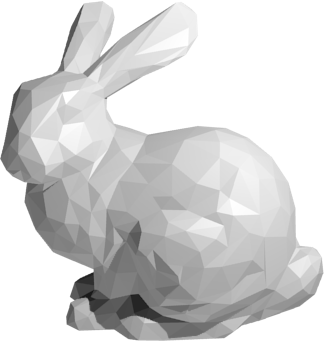
\includegraphics[width=\textwidth]{figures/lod/decimation2.png}
    \end{subfigure}
    ~ %add desired spacing between images, e. g. ~, \quad, \qquad, \hfill etc. 
    %(or a blank line to force the subfigure onto a new line)
    \begin{subfigure}[b]{0.2\textwidth}
        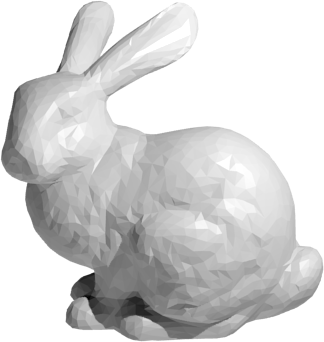
\includegraphics[width=\textwidth]{figures/lod/decimation1.png}
    \end{subfigure}
    \caption{A range of predefined meshes with increasing resolution}
    \label{fig:dlod}
\end{figure}

At run time, the main objective is to select one (or generate) a suitable representation. This approach does not provide any means of dealing with large scale datasets, which makes it unsuitable for globe rendering (ref virtual globes).


\subsection{Continuous Level of Detail}
The continuous LOD (CLOD) approach represents a model in a way that allows the resolution to be selected arbitrary. This is usually implemented by a base mesh combined with a sequence of operations that successively changes the level of detail of the model. Two typical such operations are ``edge collapse'' (removes two triangles from the mesh) and its inverse, ``vertex split'' (adds two triangles to the mesh) are illustrated in Figure \ref{fig:clod}.

\begin{figure}
    \centering
    \begin{subfigure}[b]{0.2\textwidth}
        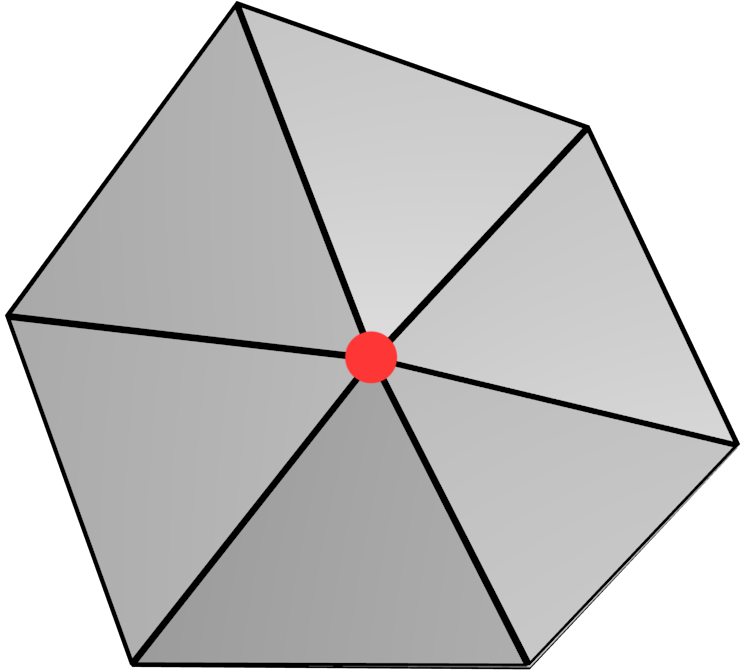
\includegraphics[width=\textwidth]{figures/lod/vertex_split1.png}
    \end{subfigure}
    ~ %add desired spacing between images, e. g. ~, \quad, \qquad, \hfill etc. 
      %(or a blank line to force the subfigure onto a new line)
    \begin{subfigure}[b]{0.2\textwidth}
        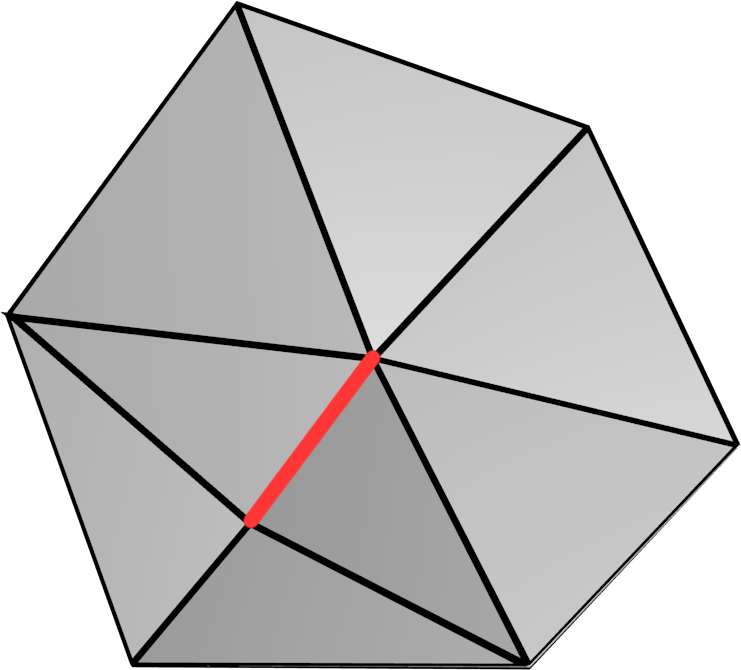
\includegraphics[width=\textwidth]{figures/lod/vertex_split2.png}
    \end{subfigure}
    \caption{Edge collapse in continous LOD}
    \label{fig:clod}
\end{figure}

According to Cozzi and Ring \cite[p. 368]{cozzi11} CLOD has previously been the most popular approach for rendering terrain at interactive rates, with implementations such as Real-time Optimally Adaptive Mesh (ROAM). The main reason CLOD algorithms are not widely employed these days is due to the increase in triangle throughput on modern GPUs, causing the CLOD operations done on the CPU in many cases to act as a bottleneck for the rendering time.

A special branch of CLOD worth mentioning is the so called infinite LOD. In this approach the terrain is represented by a mathematical function - an implicit surface. These functions can be defined by fractal algorithms and produce complex characteristics, or they can define simple geometric shapes such as spheres or ellipsoids. As every point on these types of surfaces are precisely defined, triangle meshes can be generated with no limit on the level of detail. This approach is not suitable for incorporating real world data, but it is used by terrain engines such as Outerra and Terragen to procedurally generate terrain at any desired level of detail \cite{outerraprocedural09}. 

\subsection{Hierarchical Level of Detail}
Hierarchical Level of Detail (HLOD) can be seen as a generalization of DLOD. HLOD algorithms operates on hierarchically arranged, predefined chunks of the full model. Each chunk is processed, stored and rendered separately. By doing this, HLOD approaches tackles the weaknesses of CLOD, essentially by doing the following.

\begin{enumerate}
    \item Reduce processing time on CPU: The only CPU task that HLOD algorithms has to deal with during runtime is to select a suitable subset of the predefined chunks for rendering. This is a relatively fast procedure in contrast to iteratively applying changes to the raw geometry, as done in CLOD.
    \item Reduce the data traffic to GPU: Data is uploaded to the GPU in larger batches but not very often, since the data is static and GPU caching can be done. With CLOD, the geometry data is updated on a per-frame basis, and can't be cached on the GPU. Being able to perform GPU caching allow HLOD to better minimize the traffic to the GPU.
\end{enumerate}

HLOD uses spatial hierarchical data structures such as quadtrees or octrees for storing the chunk data. The root node of the tree holds a full representation of the model at its lowest level of detail a one single chunk. At successive levels, the model is represented at a higher level of detail but divided up into several chunks. This concept is illustrated in Figure \ref{fig:hlod}.

\begin{figure}[htbp]
    \centering
    \begin{subfigure}[bt]{0.4\textwidth}
        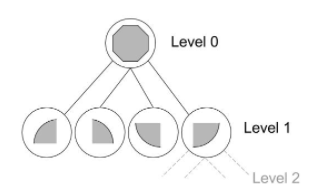
\includegraphics[width=\textwidth]{figures/lod/hlod_tmp.png}
    \end{subfigure}
    \caption{HLOD using a quadtree.}
    \label{fig:hlod}
\end{figure}

Generally, selecting all the chunks at a specific level in the tree yields a complete representation of the model. Furthermore, chunks may be selected from different levels for different parts of the model and still yield a full representation of the model. This allows for view dependent rendering of the model. Algorithm chunk selection describes pseudo code for recursively rendering the full model at view dependent level of detail.

\begin{algorithm}[htp]
  \SetKwFunction{RenderLOD}{}
  \SetKwProg{myalg}{RenderLOD}{}{}
  \myalg{\RenderLOD{Camera C, ChunkNode N}}{
  \eIf{ErrorMetric($C$, $N$) < threshold}{
        Render($N$, $C$)
    }{
        \For{$child$ \textbf{in} $children(N)$}{
            RenderLOD($child$, $C$)
        }
    }
  }{}
  \caption{Algorithm with procedure}
\end{algorithm} 

This example uses a depth first approach for rendering of chunks. Other common schemes for traversing the hierarchy are breadth first and inverse breadth first.

The algorithm traverses the tree and calculates an error metric at each node with respect to the current camera position. If the calculated error is larger than a certain threshold, the algorithm recursively repeats the procedure for all the chunk's children, which has higher level of detail. This general scheme can be used for rendering one-dimensional curves (using a binary tree structure), two-dimensional surfaces (using a quadtree) or volumes (using an octree).

Another key feature of HLOD as opposed to DLOD and CLOD is that it can naturally be integrated with out-of-core rendering, as chunks can be loaded into memory on-demand and thrown away when not needed.

%%%%%%%%%%%%%%%%%%%%%%%%%%%%%%%%%%%%%%%%%%%%%%%%%%%%%%%%%%%%%%%%%%%%%


\section{Level of Detail Algorithms for Globes}
A number of different LOD algorithms has been introduced for the purpose of globe rendering. Two common algorithms used are Chunked LOD and Geometry Clipmaps, as pointed out by Cozzi and Ring\cite{cozzi11}.

\subsection{Chunked LOD}
The Chunked LOD method fits into the category of a HLOD system and works by breaking down the surface of the globe into a quadtree of chunks. There are several different tiling schemes that can be used for spatially organizing the chunks. Some tiling schemes are defined as the ellipsoidal tessellation methods described under ``Tessellating the Ellipsoid''. 

\begin{figure}[htbp]
    \centering
    \begin{subfigure}[bt]{0.4\textwidth}
        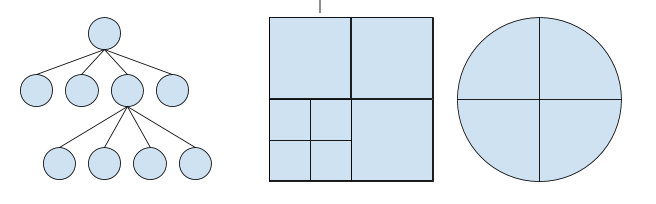
\includegraphics[width=\textwidth]{figures/chunkedlod/chunkedlodglobe.png}
    \end{subfigure}
    \caption{Chunk LOD for a globe}
    \label{fig:chunkedlod}
\end{figure}

Figure \ref{fig:chunkedlod} demonstrates the layout of chunks as they are mapped in geographic coordinates onto an ellipsoid representation of a globe.

\subsubsection{Chunks}
Chunks should store the following data:

\begin{enumerate}
    \item A mesh defining the terrain geometry (positions, normals, uv-coordinates). 
    \item A monotonic geometric error, based on the vertices distances to the fully detailed mesh. The children of a chunk should always have a smaller geometric error as they can better fit the highest level of detail model.
    \item A known bounding volume encapsulating the mesh and optimally all the chunk's children. This is used along with the geometric error metric when selecting suitable chunks for rendering.
\end{enumerate}

Depending on the implementation of the chunked LOD algorithm, these properties can be either calculated on the fly or preprocessed as suggested by Cozzi and Ring\cite[p. 447]{cozzi11}. Furthermore, the chunk mesh must fulfill two important requirements: 

\begin{enumerate}
    \item Have vertices defined in each corner of the mesh
    \item Have defined edges along its sides such that when two adjacent chunks are rendered next to each other, there is no gap in between them. See subsection Cracks below for more about this topic
\end{enumerate}

Cozzi and Ring suggests rectangular chunk meshes, although triangular tiling schemes (such as HTM) can also be used \cite{htm}.

\subsubsection{Selection}
There are different ways of selecting chunks for rendering, based on different ways of calculating an error metric for each chunk. (See Algorithm chunk selection in HLOD section). As an example, a very simple view-dependent error metric could use the chunk size divided by the distance between the camera and the chunk. If the ratio is larger than a certain threshold, the algorithm should instead consider each of the chunk's children by splitting the chunk into four. Another approach is to consider the actual visual effect on the screen. With a geometric error stored in each chunk, it is possible to calculate a maximum screen space error in pixels with respect to the current camera view. [Cozzi and Ring] This gives the user the convenience of being able to specify a maximum pixel error threshold.

\subsubsection{Culling}
An important thing to consider when dealing with chunks of a virtual globe is the fact that the chunks that are selected for rendering might not actually be visible on the screen. Needless to say, this is a waste of computational power and by eliminating these unnecessary draw calls, the performance of the globe renderer can be increased.

\paragraph{Camera frustum culling} This is done by testing a bounding box of the chunk for intersection with the camera frustum. If the chunk is completely outside the frustum, the chunk can safely be culled as it will not be visible in the rendered image. See Figure \ref{fig:frustumculling}.

\begin{figure}[htbp]
    \centering
    \begin{subfigure}[bt]{0.4\textwidth}
        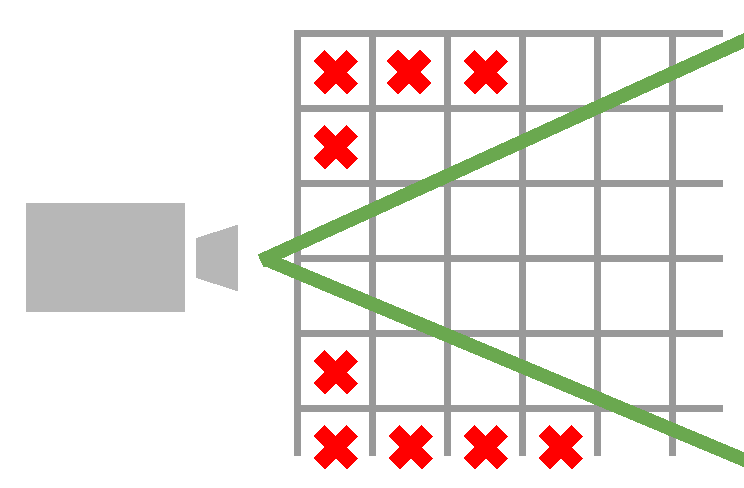
\includegraphics[width=\textwidth]{figures/chunkedlod/frustumculling.pdf}
    \end{subfigure}
    \caption{Frustum culling}
    \label{fig:frustumculling}
\end{figure}

\paragraph{Horizon culling} Even after camera frustum culling there are chunks that still do not contribute to the rendered image. Figure \ref{fig:horizonculling} illustrates that most of a globe is actually invisible to any observer. This can be used as a basis for culling some of the remaining chunks. 

\begin{figure}[htbp]
    \centering
    \begin{subfigure}[bt]{0.4\textwidth}
        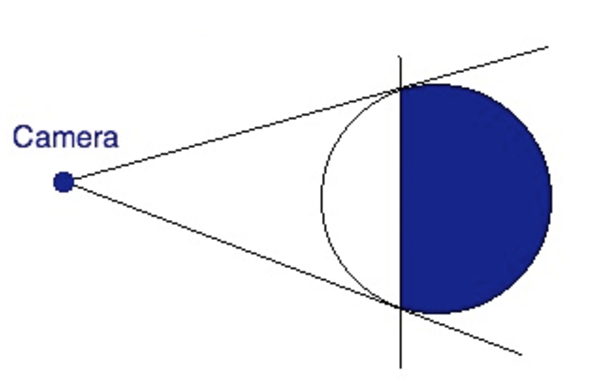
\includegraphics[width=\textwidth]{figures/chunkedlod/horizonculling.png}
    \end{subfigure}
    \caption{Horizon culling}
    \label{fig:horizonculling}
\end{figure}


\subsubsection{Switching}
Even with sophisticated methods for selecting and culling chunks, users of a globe rendering system will notice ``popping'' effects as chunks are splitted and merged. Even when chunks can be selected in a way that guarantees a maximum pixel error per vertex, the fact that full areas of multiple triangles are replaced all at once causes a drastic change in the rendered view. Even when the updates are small per vertex, the update of whole chunk areas may be easily noticed. This is what is referred to as popping.

Minimizing popping artifacts are typically done by smoothly transitioning between levels over time. Cozzi and Ring suggest an approach where along with each vertex, a delta offset is also stored\cite[p. 451]{cozzi11}. This delta offset stores the difference between the chunk itself and the same region within the parent chunk. Using this difference, new vertices can be placed on already defiend edges, and then interpolated into their actual positions. Figure switch below illustrates the idea.

\begin{figure}[htbp]
    \centering
    \begin{subfigure}[bt]{0.7\textwidth}
        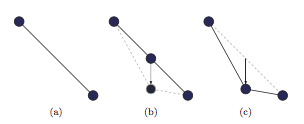
\includegraphics[width=\textwidth]{figures/chunkedlod/switching.png}
    \end{subfigure}
    \caption{a) An edge at chunk level i-1. b) The same edge after level i has been selected. c) The new vertex is interpolated into its true place.}
    \label{fig:lodswitch}
\end{figure}

The interpolation parameter can be based on the distance to the camera or time based animation.

\subsubsection{Cracks and skirts}
As chunks are tiled and rendered next to each other, it is desireable to make the borders between chunks as unnoticeable as possible. Even though the chunk meshes are generated according to the requirements mentioned in the Chunk subsection above, it is not possible to guarantee a watertight edge between two adjacent chunks of different LOD. Where adjacent chunks have different detail level, so called T-junctions till emerge. These T-junctions cause cracks between the chunks as an unwanted visual artifact.

The easiest way to tackle this issue is not to try to remove the cracks, but instead try to hide them. The most common approach hides the cracks by simply adding an extra layer of vertices to the sides of sides of the mesh. This extra layer of vertices, which are also known a skirt, is offset down vertically, as illustrated in figure \ref{fig:skirts}. 

By adding skirts to the chunk meshes, the model will not be rendered with visible holes in it. Instead, the holes will be filled up with textured triangles.

\begin{figure}[htbp]
    \centering
    \begin{subfigure}[bt]{0.4\textwidth}
        
\includegraphics[width=\textwidth]{figures/chunkedlod/skirts_without.png}
        \caption{No skirts.}
    \end{subfigure}
    \begin{subfigure}[bt]{0.4\textwidth}
        
\includegraphics[width=\textwidth]{figures/chunkedlod/skirts_with.png}
        \caption{Skirts}
    \end{subfigure}
    \caption{Chunks with skirts hide the undesired cracks between them.}
    \label{fig:skirts}
\end{figure}


\subsection{Clipmaps Geometry}
A clipmap texture is a dynamic mip map where each image in the so called clipmap stack is clipped down to a constant size. This reduces the amount of memory of the whole texture to increase linearly instead of exponentially with the number of overlays for LOD textures. However, clipmaps demands updating as the focus point of the texture moves . Figure \ref{fig:flipmapmipmap} a shows the difference between the amount of texture data stored in a regular mip map compared to a clipmap.

\begin{figure}[htbp]
    \centering
    \begin{subfigure}[bt]{0.8\textwidth}
        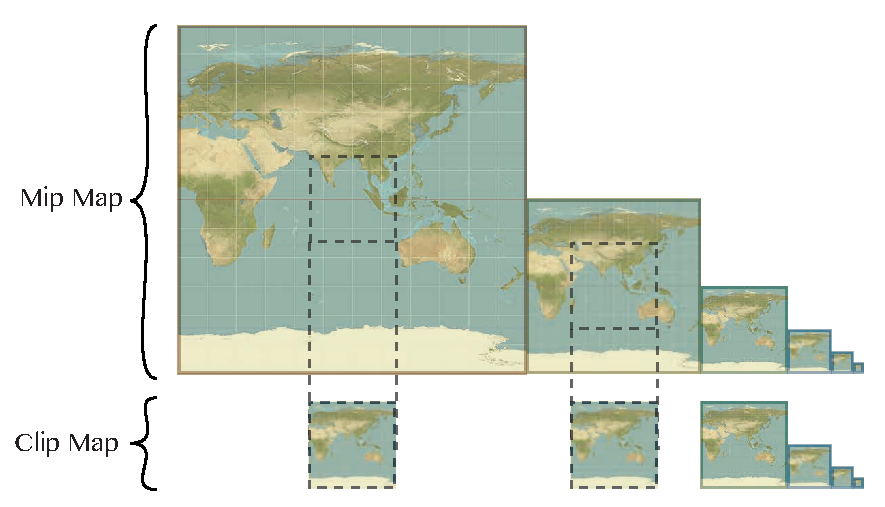
\includegraphics[width=\textwidth]{figures/geometryclipmap/clipmap_mipmap.pdf}
    \end{subfigure}
    \caption{Comparison of MipMaps and ClipMaps}
    \label{fig:clipmapmipmap}
\end{figure}

The Idea of clipmaps can be applied not only to textures but also to geometries. By representing a terrain by a stack of clipmap geometries of different size, the resolution increases closer to the focus point which can be the horizontal position of a virtual camera, see figure fnöske b. The position of each of the levels of the clip map geometries snaps to a discrete coordinate grid with cell sizes equal to the distance between two adjacent vertices.

Geometry clipmaps limits the terrain representation to be in the form of height maps. This is because the clipmap geometry moves around when the focus point changes and since the underlying terrain should not follow the camera position, the clipmap geometries requires vertex shader texture fetching. The texture coordinates are offset as the geometry clipmap moves to follow the focus point.

\begin{figure}[htbp]
    \centering
    \begin{subfigure}[bt]{0.6\textwidth}
        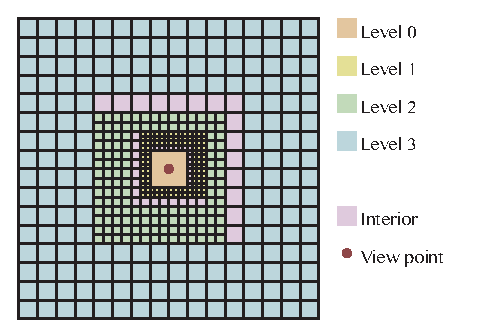
\includegraphics[width=\textwidth]{figures/geometryclipmap/clipmap_geo.pdf}
    \end{subfigure}
    \caption{Geometry Clipmaps}
    \label{fig:clipmapgeometry}
\end{figure}

One of the main selling points for geometry clipmaps is the decrease in CPU workload and the increase in GPU triangle throughput. There is no need to traverse a hierarchical structure such a quadtree. The number of draw calls will decrease to the number of clip maps instead of the number of chunks which is often larger. The framerate will also be relatively consistent if the number of layers in the clipmap stack remains constant.

\subsubsection{2D Grid Geometry Clipmaps}
Using geometry clipmaps to achieve dynamic level of detail for a height mapped grid was proposed by Dimitrijevi\'{c} and Ran\v{c}i\'{c} \cite{dimi15}. The method is limited to rendering of equirectangular grids. It works well when the viewer has a constant distance to the surface and when the scales are small enough to disregard the curvature of the globe.

When considering the ellipsoidal shape of a globe, the clipmap grid can be represented in geographic coordinates mapped on an ellipsoid where the map texture coordinates in the longitudinal direction wraps around the anti meridian. Rendering the clipmap close to the poles however will lead to polar pinching which breaks the globe, see figure \ref{fig:mipclip}.

\begin{figure}[htbp]
    \centering
    \begin{subfigure}[bt]{0.35\textwidth}
        \includegraphics[width=\textwidth]{figures/geometryclipmap/clipmap1.png}
        \caption{Near the equator}
    \end{subfigure}
    \quad
    \begin{subfigure}[bt]{0.35\textwidth}
        \includegraphics[width=\textwidth]{figures/geometryclipmap/clipmap2.png}
        \caption{Near a pole}
    \end{subfigure}
    \caption{Geometry Clipmaps on a geographic grid cause pinching effect around the poles, which needs to be handled explicitly.}
    \label{fig:mipclip}
\end{figure}

Clipmap grids can also be used to model a spherical cube representation of a globe to avoid polar issues. This requires six clipmap partitions; one for each side of the cube.

\subsubsection{Spherical Clipmaps}
Spherical clipmaps takes advantage of the fact that no observer will ever see more than half a globe at any time instance. The vertices of the clipmap are described in polar coordinates with the center of the grid always following the camera position. The coordinates of the vertices will therefore not have any correspondence to texture coordinates which is why the algorithm is not widely adopted\cite{dimi15}. 

\subsubsection{Ellipsoidal Clipmaps}
Dimitrijevi\'{c} and Ran\v{c}i\'{c} introduces ellipsoidal clipmaps as a level of detail rendering method for globes \cite{dimi15}. It uses a geographic grid for the polar regions of the globe and solves the polar issues with the use of polar caps. The advantages compared to spherical cube clipmaps is that it uses the well known geographic map projection and reduces the number of geometry clipmap partitions from six to two. The globe is divided into one equatorial region and two polar regions. If the distance is close enough to the globe (3,000 km above the surface for the Earth), a maximum of two partitions is needed at any time \cite{dimi15}.

The area distortion and the aspect distortion of the map projection of the ellipsoidal clipmap method is low compared to cube map projections but requires extra care to hide the discontinuities that appear at the edges between the equatorial and polar partitions \cite{dimi15}.

The most generally used level of detail algorithms of today are chunked LOD and varieties of geometry clipmaps. AAA and BBB compares the algorithms and gives the advantages and disadvantages depending on the needs of the globe browsing software. A summation of the comparison is shown in table jox. The differences were considered when choosing the algorithm for the implementation, however noting that some of the properties can be shared between the two algorithms to more effectively meet the objectives.

The main differences between the Chunked LOD approach and Geometry Clipmaps are summarized and presented in Table \ref{table:lodcomparison} \cite[p. 464]{cozzi11}.
\begin{center}
  \begin{table}
  \caption[]{Comparing geometry clipmapping and chunked LOD}
    \label{table:lodcomparison}
  \begin{tabular}{| r | c | c |}
    \hline
                            & \textbf{Geometry Clipmaps} & \textbf{Chunked LOD} \\ \hline

    Preprocessing           & Minimal           & Extensive \\
    Mesh Flexibility        & None              & Good \\
    Triangle Count          & High              & Lower \\
    Ellipsoid Mapping       & Challenging       & Straightforward \\
    Error Control           & Poor              & Excellent \\
    Frame-Rate Consistency  & Excellent         & Poor \\
    Mesh Continuity         & Excellent         & Poor \\
    Terrain Data Size       & Small             & Large \\
    Legacy Hardware Support & Poor              & Good \\
    \hline
  \end{tabular}
  \end{table}
\end{center}

%%%%%%%%%%%%%%%%%%%%%%%%%%%%%%%%%%%%%%%%%%%%%%%%%%%%%%%%%%%%%%%%%%%


\section{Large Scale Map Datasets}

Global maps with high level of detail can easily become too large to be stored and read locally on a single machine. A common way of storing large maps is by representing them using several overviews. An overview is a map representing the same geographical area as the original map but containing only one fourth as many pixels just like a lower level of a mip map texture. Figure \ref{fig:overview} shows how the size of the maps in raster coordinates decreases with the overview number.

\begin{figure}[htbp]
    \centering
    \begin{picture}(130,60)
        \put(0,0){\includegraphics[width=0.5\textwidth]{figures/overview.pdf}}
        \put(-50,50){Overview:}
        \put(45,50){0}
        \put(127,50){1}
        \put(176,50){n}
        \put(-5,25){$y$}
        \put(45,-5){$x$}
    \put(100,35){$\frac{y}{2}$}
    \put(127,15){$\frac{x}{2}$}
    \put(155,37){$\frac{y}{2^n}$}
        \put(176,25){$\frac{x}{2^n}$}

        \label{fig:proj_equirectangular}
    \end{picture}
    \caption{The size of the map is decreasing exponentially with the overview.}
    \label{fig:overview}
\end{figure}

The physical disk space of large global map datasets is often measured in terabytes or even petabytes. In order to deal with such large datasets, web based services allow users to specify only parts of the map to download at a time. This is an important aspect in the out of core rendering required for globe visualization.

\subsection{Web Map Services}

To standardize web requests for map data, the Open GIS Consortium (OGS) specified a web map service interface \cite{wms06} and from that, specifications of several other map service interfaces have followed. The most common standards are Web Map Service (WMS), Tile Map Service (TMS) and Web Map Tile Service (WMTS). Some more specific examples of WMS-like services are WorldWind, VirtualEarth and AGS. The last three are not covered in this thesis.

\subsubsection{WMS}

The WMS interface produces maps as image files with well defined geographic and dimensional parameters. The image files can have different format and compression depending on the provider. A WMS server has the ability to dynamically produce map patches of arbitrary size which puts some load on the server side \cite{wms06}. The basic elements supported by all WMS providers are the \emph{GetCapabilities} and the \emph{GetMap} operations. \emph{GetCapabilities} gives information about the available maps on the server and their corresponding geo referenced metadata. The \emph{GetMap} operation returns the map or a part of the map as an image file.

The structure of a WMS request using HTTP GET is of the form \\ \texttt{http://host\lbrack:port\rbrack/path\lbrack?\{name\lbrack=value\rbrack\&\}} where the name and value pairs are defined for each operation by the standard \cite{wms06}. For example, setting the parameter \texttt{BBOX=-180,-90,180,90} specifies the size of the map in geo referenced coordinates while the parameters \texttt{WIDTH} and \texttt{HEIGHT} specifies the requested image in raster coordinates. All name and value pairs for the \emph{GetMap} request are defined under the reference \cite{wms06}.

\subsubsection{TMS}

Tile Map Service (TMS) was developed by the Open Source Geospatial Foundation (OSGeo) as a simpler solution to requesting maps from remote servers. The specification uses integer indexing for requesting specific precomputed tiles instead of letting the server side spend time on producing maps of arbitrary dimensions. The TMS interface is similar to WMS but simpler and it does not support all the features of WMS \cite{tms}.

\subsubsection{WMTS}

Web Map Tile Service is the standard by OGS that requires tiled requests. It supports many of the features of WMS but, similar to TMS, removes the load of image processing from the server side and instead forces the client to handle combination and cutouts of patches if required. The standard specifies the \emph{GetCapabilities}, \emph{GetTile} and \emph{GetFeatureInfo} operations. These operations can be requested with different message encodings such as Key-Value Pairs, XML messages or XML messages embedded in SOAP envelopes \cite{wmts10}.

\subsubsection{Tiled WMS}

Before the WMTS standard was developed, some servers had already embarked on the tiled requests by limiting the valid bounding boxes to values that only produce precomputed tiles. These services can be referred to as Tiled WMS and are nothing more than specified WMS services where the server limits the number of valid requests \cite{wmts10}.

\subsection{Georeferenced Image Formats}

There are several different standards for handling image data used in GIS softwares. Some common file formats with image data and/or geo referenced information that are used in the below mentioned imagery products are:

\begin{itemize}  
\item \emph{GeoTIFF}, TIFF image with the extension of containing geo referenced metadata. 
\item \emph{IMG}, Image file format with geo referenced metadata. 
\item \emph{JPEG2000}, Geo referenced image format with lossy or lossless compression.
\item \emph{CUB}, Geo referenced image file standard created by ISIS (Integrated Software for Imagers and Spectrometers)
\end{itemize}

\subsection{Available Imagery Products}

There are several organizations working on gathering GIS data that can be visualized as flat 2D maps or projected on globes. Many of them provide their map data through web map services. However, they are often defined in different formats and sometimes available only as downloadable image files.

\subsubsection{Earth}

\textbf{NASA Global Imagery Browse Services (GIBS)} provides several global map datasets with information about Earth's changing climate. The two satellites Aqua and Terra orbit the Earth and are continuously measuring multi band quantities such as corrected reflectance and surface reflectance along with a range of scientific parameters such as surface- and water temperatures, ozone, carbon dioxide and more. Many of the GIBS datasets are updated daily or monthly so that changes can be seen over time. Map tiles are downloaded through a TMS interface and a date and time parameter can be set if the dataset is temporal.

\textbf{Environmental Systems Research Institute (ESRI)} is the provider of the software ArcGIS that lets their users create and publish map data through different types of web map services. There are a lot of free maps to use; not only for Earth but other globes are covered too. ESRI supports a web publication interface where web maps can be searched and studied in an online map viewer. Many of the maps are given in mercator coordinates since they are meant to be viewed projected on a flat surface such as a screen where aspect ratio should be preserved.

\textbf{National Oceanic and Atmospheric Administration (NOAA)} for the U.S. Department of Commerce gathers and provides weather data of the US that are hosted through different web map services using the ArcGIS online \cite{arcgis} interface by ESRI.

\textbf{Open Street Map} is a free global map of streets and roads created and editable by the public and usable by anyone through a TMS interface. The map uses the web mercator projection.

\subsubsection{Mars}

The first global color images taken of Mars were by the two orbiters of the Viking missions that launched in late 1975. NASA Ames worked on creating the Mars Digital Image Models (MDIM) by blending a mosaic of images taken by the orbiters. United States Geological Survey (USGS) provides downloading of image files in CUB or JPEG2000 format. The maps are still the highest resolution global color maps of the planet.

NASA's Mars Reconnaissance Orbiter (MRO) is a satellite that has been orbiting Mars since 2006, gathering map data by taking pictures of the surface. The satellite has three cameras; the Mars Color Imager (MARCI) for mapping out daily weather forecasts, the Context camera (CTX) for imaging terrain and the High Resolution Imaging Science Experiment (HiRISE) camera for mapping out smaller high resolution patches covering limited surface areas of interest. NASA enables downloading of local patches and digital elevation models (DEMs) and grayscale images taken by the CTX and the HiRISE cameras in IMG and GeoTIFF formats.

\subsubsection{Moon}

The Lunar Mapping Modeling Project (LMMP) is an initiative by NASA to gather and publish map data of the Moon from a vast range of lunar missions. The Lunar Reconnaissance Orbiter (LRO) is a satellite orbiting the moon and gathering map data for future landing missions. These maps have been put together into global image mosaics as well as DEMs. Most global maps from LMMP can be accessed via the onmoon web interface \cite{onmoon}.


\chapter{Implementation}
The virtual globe rendering system was implemented as a separate module, programmed in C++ for OpenSpace which, if desired, can be opted out when building the software in CMake. The implementation defines a namespace with all the necessary data structures, classes and functionality specifically related to globe rendering. The basic structure of a renderable globe with its necessary components is illustrated as a UML diagram in figure \ref{fig:renderableglobe}.

\begin{figure}[htbp]
    \centering
    \begin{subfigure}[bt]{0.8\textwidth}
        \includegraphics[width=\textwidth]{figures/implementation/renderable_globe.pdf}
    \end{subfigure}
    \caption{Overviewing class diagram of RenderableGlobe and its related classes.}
    \label{fig:renderableglobe}
\end{figure}

The base of the globe renderer uses a modified version of Cozzi and Rings Chunked LOD algorithm. The globe is tessellated as an ellipsoid with a geometrical grid using geodetic map projection.

The full LOD rendering system required several components of different complexity to be implemented. These along with their puruposes are listed below.

\begin{enumerate}
	\item \textbf{Reference Ellipsoid}% - A small independent component for geometry calculations.
	\item \textbf{Chunked LOD}% - Hierarchically arranges Chunks in a quadtree where each Chunk represents a geographical region and can be rendered individually.
	\item \textbf{Reading and Tiling Image Data}% - A large component that takes care of concurrent texture fetching, georeferencing and tiling up textures to fit chunks. 
	\item \textbf{Providing Tiles}% - How to access different types of tiles.
	\item \textbf{Mapping Tiles onto Chunks}% - 
	\item \textbf{Managing Multiple Data Sources}% - Organizes different texture layers into categories and makes the texture data accessible for rendering. 
	\item \textbf{Chunk Rendering}% - 
\end{enumerate}



\section{Reference Ellipsoid}
The reference ellipsoid class was implemented to handle all geographic related calculations.  These calculations include conversions between geodetic and cartesian coordinates and different kinds of projections onto the ellipsoid surface. These calculations are sped up by internal caching of a range of precalculated values. Cozzi and Ring provide a complete reference on the implementation \cite[p. 17]{cozzi11}.

The Ellipsoid uses several geographically related classes, which were used in multiple places within the implementation. These are:
\begin{enumerate}
	\item Angle - Handles angle related arithmetics, normalizations and abstract away units (degrees and radians)
	\item Geodetic2 - Represents a 2D geodetic coordinate (latitude, longitude)
	\item Geodetic3 - Represents a 3D geodetic coordinate (latitude, longitude, altitude)
	\item GeodeticPatch - Represents a rectangular region in geodetic space
\end{enumerate}

\section{Chunked LOD}
The base of the chunked LOD algorithm revolves around the self updating chunk tree. The chunk tree is a data structure built up of chunk nodes which have the ability to split or merge dynamically. Besides storing four chunk node children, each chunk node stores a Chunk.

\subsection{Chunks}
As opposed to the definition of chunks in the background section \ref{section:chunkedlodbacground}, this implementation of chunks is very lightweight - it does not store any texture or triangle mesh data. Instead, it stores the information needed to query texture tiles from local in-memory caches. In the implementation suggested by Cozzi and Ring, terrain triangle meshes are stored in each chunk. In the case of this implementation however, all terrain is rendered using height mapped vertex grids. Thus there is no need for each chunk to store their own vertex arrays. Instead they can simply share one single instance of a vertex grid within a whole chunk tree. This means that vertices need to be offset by height mapping on the GPU.

The most important part of the chunked LOD algorithm is the ability to dynamically select which chunks to split or merge. 

\subsection{Chunk Selection}
The chunk tree is automatically reshaped depending on the virtual camera. A Chunk node splits, merges or remain the same depending on the chunk's error metric for the current LOD. Three different approaches for calculating the error metric were implemented.

\subsubsection{By Distance}
By letting the error depend on the distance between the closest point on the chunk, an the camera $d$ as in Equation \ref{eq:loddistance}, the size of the chunks in screen space stays more or less constant.

\begin{equation}
	\label{eq:loddistance}
	e = l - log_2(\frac{s}{d})
\end{equation}
Where $e$ is the error, $l$ is the current level of the chunk, $s$ is a LOD scaling factor and $d$ is the distance between the closest point of the chunk and the camera. The closest point of the chunk can be either a corner or a point along one of the chunk edges. Using this distance as an error metric leads to bigger chunks farther from the camera where less detail is needed.


\subsubsection{By Projected Area}
Another error metric is the area that the chunk take up on the screen. The bigger the area, the higher the error. 

The error must not be dependent of the direction of the camera. This is because a chunk rendered on a multi screen display should not have different errors between two or more screens which might lead to different levels and tearing between screens. Therefore the chunk is projected on a unit sphere and not a view plane which would lead to view direction dependent error metrics.

\begin{figure}[htbp]
    \centering
    \begin{subfigure}[bt]{0.5\textwidth}
        \includegraphics[width=\textwidth]{figures/implementation/chunklod/projectedarea.png}
    \end{subfigure}
    \caption{Chunk are projected onto a unit sphere}
    \label{fig:chunkprojarea}
\end{figure}

The projected area is a solid angle approximated by extracting three points on the chunk and projecting them on a unit sphere centered in the camera position. The three points define the closest of the four center triangles on the chunk, see Figure \ref{fig:chunkprojarea}. It is important that the triangle chosen for approximating the projected area can never have two vertices on the same upper or lower most edge. Such triangles (colored gray in Figure \ref{fig:chunkprojarea}) may have null areas at the poles, thus cannot be used to approxate the area of the full chunk.

The actual approximated solid angle is the projected triangle area multiplied by eight to accommodate a full chunk. This area is then subtracted by a constant value and scaled by a LOD scale factor to give similar LOD scaling as the distance dependent chunk selection.

\subsubsection{By Available Tile}
Splitting a chunk will not result in higher level of detail unless the corresponding higher level of detail tile data is also currently available for rendering. Therefore, the growth of the chunk tree can be limited by checking if there is any tile data there in the first place. This is useful in two scenarios:

\begin{enumerate}
\item Rendering of sparse map datasets which contain geographical regions where there are no data
\item Rendering of map datasets which are queried from remote servers - there will always be some delay where the queried map data is not yet available
\end{enumerate}

Being able to limit the chunk tree in these two scenarios, unnecessary chunk rendering calls can be avoided.

\subsection{Chunk Culling}
Given a chunk tree with chunks selected based on the camera position, each chunk can be tested using chunk cullers to determine if they are ``cullable'' and therefore can be set to invisible so that the chunk renderer will not bother in rendering them. The two implemented chunk cullers are the frustum culler and the horizon culler. They both rely on - and have access to - minimum and maximum values of the chunk's height maps. 

\subsubsection{Frustum Culling}
The frustum culling is implemented by first calculating a convex bounding polyhedron for the chunk to be tested. The bounding volume is calculated on the fly and takes into account any enabled height maps used to displace the vertices, making sure it fully encapsulates the displaced chunk vertices. The polyhedron is built up of eight vertices which are transformed to normalized device coordinates (NDC). Once in NDC, an axis aligned bounding box (AABB) for the vertices is extracted. This AABB can then be tested against the screen bounds to determine if the chunk is outside the camera's field of view, and thus can be cullable. This is illustrated in Figure \ref{fig:frustumculling}.

\begin{figure}[htbp]
    \centering
    \begin{subfigure}[bt]{1.0\textwidth}
        \includegraphics[width=\textwidth]{figures/implementation/chunklod/frustumculling.pdf}
    \end{subfigure}
    \caption{Frustum culling algorithm. The chunk cannot be frustum culled.}
    \label{fig:frustumculling}
\end{figure}

\subsubsection{Horizon Culling}
Given an object in position $\vec{p}$ with a bounding radius $r$, it can be determined if it is completely behind the globe's horizon or not. The calculations are simplified by approximating the globe as a sphere using the minimum radius $r_g$ of its ellipsoid. Using the minimum radius and not a bigger number ensures that false occluding (chunks marked as invisible actually being visible) is not possible \cite[p. 393]{cozzi11}. The minimum allowed distance $l$ to the object can be calculated as the distance to the horizon $l_h$ added to the minimum allowed distance to the object from the horizon $l_m$. See figure \ref{fig:horizonculling}. Once the minimum allowed distance is calculated it can be compared to the actual distance to the object to determine if it is cullable or not.

\begin{figure}[htbp]
    \centering
    \begin{picture}(130,130)
        \put(0,0){\includegraphics[width=0.4\textwidth]{figures/implementation/chunklod/horizonculling.pdf}}
        \put(60,145){$l_h$}
        \put(115,125){$l_m$}
        \put(135,95){$r$}
        \put(70,95){$r_g$}
        \put(130,80){$\vec{p}$}
        
    \end{picture}
    \caption{Horizon culling.}
    \label{fig:horizonculling}
\end{figure}

When culling chunks, the closest position on the chunk is used as the position $\vec{p}$ and the bounding height value as $r$.

\section{Reading and Tiling Image Data}
Fetching the right texture and preparing it for rendering onto chunks is a fairly complicated process. Before digging into the details of this process, there are three concepts that need to be established, as they will be referred to throughout the description of the texture pipeline. These are:

\begin{enumerate}
	\item \textbf{Tile index} - A tuple of three integers $(level, x, y)$ indexing a specific map region on the globe.
	\item \textbf{Raw tile} - A texture carved out to fit the geographical region of a specific chunk, along with some meta data. Each raw tile is associated with a tile index. They can be instantiated concurrently.
	\item \textbf{Tile} - Like a raw tile, but the texture data is uploaded to the GPU and ready to use for rendering (unless it has a status not equal to ``OK''). As opposed to raw tiles, tiles rely on an OpenGL context and must therefore be initialized on the rendering thread.
\end{enumerate}

All chunk height and texture data are represented using tiles. Tiles are created on the client side (i.e. in OpenSpace) on the fly when they are needed. As the pixel data may need to be read from disk or even requested from remote servers, the whole tile preparation pipeline was implemented to be executed on separate threads in order to avoid blocking the rendering thread with image data reads. 

During the iterative process of developing the texture tile pipeline, three layers of abstraction were introduced in order to deal with the fairly high complexity. These are listed in Table \ref{table:tilepipeline}.

\begin{center}
  \begin{table}
  \caption[]{Abstraction layers used in the texture data pipeline}
    \label{table:tilepipeline}
  \resizebox{\textwidth}{!}{\begin{tabular}{| c | c | c | c |}
    \hline
     Layer & \textbf{Component} 	& \textbf{Responsibility} & \textbf{Input --> Output} \\ \hline 
    3 & Async Tile Dataset 	& Async RawTile fetching  & TileIndex --> RawTile \\ \hline
    2 & Tile Dataset        & Tiling, georeferencing, preprocessing & TileIndex --> RawTile \\ \hline
    1 & GDAL         		& Image formats, I/O Operations & pixel region --> pixel data \\
    \hline
  \end{tabular}}
  \end{table}
\end{center}

The subsequent sections of this chapter will cover each abstraction layer in more detail, starting from the bottom and going up the stack.

\subsection{GDAL}
Geospatial Data Abstraction Library (GDAL) is an open source library providing a uniform interface for reading, manipulating and writing geospatial data in the form of raster and vector data models \cite{gdal}. GDAL is used as an abstraction layer between all the map formats and the representation of tile datasets. It provides an interface allowing client code to specify pixel regions within a dataset to read from, independent of the underlying image format. Reading pixel data using the GDAL RasterIO interface requires a set of parameters listed below and illustrated in Figure \ref{fig:gdalio}:

\begin{enumerate}
	\item A map overview to read pixel data from (if the dataset has overviews)
	\item A pixel region within that map overview to read pixels from
	\item The raster band(s) (e.g., color channels) to read
	\item A pointer to sufficient user allocated memory where GDAL can write the output of the read operation. 
	\item The pixel region to write the outputted pixel data. (The size of the pixel data to be written may differ from the pixel region to read from, in which case GDAL will resample and interpolate the pixel data automatically.)
	\item The layout (i.e., pixel spacing, raster band spacing and line spacing)
	\item The data type to retrieve the pixel data in
\end{enumerate}

\begin{figure}[htbp]
    \centering
    \begin{subfigure}[bt]{1.0\textwidth}
        \includegraphics[width=\textwidth]{figures/implementation/pipeline/gdalio.pdf}
    \end{subfigure}
    \caption{The required GDAL raster IO parameters}
    \label{fig:gdalio}
\end{figure}

With the given input parameters shown in Figure \ref{fig:gdalio}, the resulting output would be the pixel data of the requested image region written with the pixel layout parameters to the provided memory block. The output is illustrated in Figure \ref{fig:gdalioresult}.

\begin{figure}[htbp]
    \centering
    \begin{subfigure}[bt]{0.5\textwidth}
        \includegraphics[width=\textwidth]{figures/implementation/pipeline/gdalioresult.pdf}
    \end{subfigure}
    \caption{Result of GDAL raster IO}
    \label{fig:gdalioresult}
\end{figure}

Using the RasterIO interface on an open GDAL dataset, the notion of image format is completely abstracted away. This is a great advantage which also allows GDAL to support sparse datasets. Appendix \todo{\textbf{add appendix}} goes through a detailed example of how to use GDAL as an abstraction layer for sparse, non global, datasets such as local, georeferenced, image patches and use them in our globe browsing software.

GDAL also provides the coefficients of a geo-transform which defines the mapping from raster coordinates to georeferenced coordinates.

\subsection{Tile Dataset}
Tile datasets carves out raw tiles from GDAL datasets based on a tile index. Along with the pixel data, the served raw tiles also contain some metadata. The metadata includes an error code if something went wrong during the pixel reading process and some basic information about to read pixel data, such as minimum and maximum pixel values. Figure \ref{fig:tiledataset} illustrates how the process from tile index to raw tile is carried out. There are three gray subroutines; $Get IO description$, $Read image data$ and $Calculate metadata$. These subroutines are explained below.

\begin{figure}[htbp]
    \centering
    \begin{subfigure}[bt]{0.8\textwidth}
        \includegraphics[width=\textwidth]{figures/implementation/pipeline/tiledataset.pdf}
    \end{subfigure}
    \caption{Tile datasets reads tiled pixel regions.}
    \label{fig:tiledataset}
\end{figure}

\subsubsection{Get IO Description}
The IO description contains all tile specific information needed to perform a map read request using GDAL. This includes the pixel region to read, and where to store the result. The derivation of this information is summarized in the following steps, and illustrated in Figure \ref{fig:getiodescription}.

\begin{enumerate}
\item Calculate geodetic patch from Tile index
\item Calculate the pixel coordinates for the patch in raster coordinate space
\item Calculate a suitable map overview
\item Transform pixel region to map overview
\item Add padding to the down scaled pixel region
\item Finalize the gathered data to an IO description object.
\end{enumerate}

\begin{figure}[htbp]
    \centering
    \begin{subfigure}[bt]{0.9\textwidth}
        \includegraphics[width=\textwidth]{figures/implementation/pipeline/getiodescription.pdf}
    \end{subfigure}
    \caption{Overview of the calculation of an IO description}
    \label{fig:getiodescription}
\end{figure}

% @TODO
In the scheme in Figure \ref{fig:getiodescription}, step one is performed as described in \todo{theoretical background}, equation wat is defined under section hej. 
Calculating the corresponding GDAL overview is done according to

\begin{equation}
\label{eq:overview}
Overview(level) = N - level - 1 - log_2(size_{tile} / size_{map})
\end{equation}

Where $level$ is given by the provided Tile index, $N$ is the total number of overviews in the dataset, $size_{tile}$ is a configurable constant defining the preferred pixel size of a tile and $size_{map}$ is the size of the full map in pixels. The sizes can be either along the x or y axis, but does not matter when using square tiles and maps. In the implementation x is used.

Pixel coordinates can easily be transfomed across map levels:

\begin{equation}
\label{eq:overview}
P_{n} = P_{m} * 2^{m-n}
\end{equation}

Where $n$ is the destination map overview and $m$ is the source map overview. This is used for downscaling the pixel region in step 4, where $n$ is the calculated suitable overview and $m$ is zero (i.e. the full map). 

Padding is added to the pixel region in order to do correct interpolation of pixel values across different tiles later during rendering. However, this may cause the pixel region to extend outside the map region. Therefor the last finalize step also handles wrapping of the pixel regions before return the final IO description. The wrapping used is a CPU implementation of $GL\_REPEAT$.

\subsubsection{Tile Meta Data}
As mentioned, tile datasets can be configured to calculate some metadata on the fly based on the pixel data that has been read. This information cannot be requested directly from GDAL, so this had to be implemented by explicitly looping through all the pixel values an extra time client side. In this case, raw tiles will be served with some additional information. The metadata includes minimum and maximum pixel values within the pixel data and whether or not the pixeldata contains missing-data values. Having access to minimum and maximum values for height layer tiles is required for the culling to be performed correctly since the cullers rely on having bounding boxes for the chunks.

\subsubsection{Summary}
To summarize, the implementation of TileDataset allow reading pixeldata from a GDAL dataset corresponding to a specific TileIndex, along with some metadata unless opted out. The RawTiles that are served are padded for correct interpolation avoiding visible edges in the texture between tiles. RawTiles are not available for rendering since the data is not yet on the GPU.

\subsection{Async Tile Dataset}
Async tile datasets utilize a shared thread pool and own a tile dataset. It provides a concurrent job posting interface for concurrent reads within the tile dataset. It has two important methods: 1) enqueueTileReadJob and 2) getFinishedTileReadJobs. Reading raw tiles on separate threads ensures that the render thread will not be delayed by image data requests, see Figure \ref{fig:asynctiledataset}.

\begin{figure}[htbp]
    \centering
    \begin{subfigure}[bt]{0.7\textwidth}
        \includegraphics[width=\textwidth]{figures/implementation/pipeline/asynctiledataset.pdf}
    \end{subfigure}
    \caption{Asynchronious reading of Raw tiles.}
    \label{fig:asynctiledataset}
\end{figure}

\begin{figure}[htbp]
    \centering
    \begin{subfigure}[bt]{0.7\textwidth}
        \includegraphics[width=\textwidth]{figures/implementation/pipeline/asynctiledataset2.pdf}
    \end{subfigure}
    \caption{Retrieving finished Raw tiles.}
    \label{fig:asynctiledataset2}
\end{figure}

The Async tile dataset internally keeps track of what tile indices it has enqueued and what tile index pixel regions are currently being read. If a pixel region for a specific Tile index already is currently being read, the request is simply ignored.


\section{Providing Tiles}

\subsection{Caching Tile Provider}

\subsection{Temporal Tile Provider}

\subsection{Single Image Tile Provider}

\subsection{Text Tile Provider}


\section{Mapping Tiles onto Chunks}

In the implementation of chunks suggested by Cozzi and Ring \cite{cozzi11}, chunks store the data they need for rendering by them selves. That means that as soon as a chunk has been fully initialized, it has everything it needs to be rendered. However, when dealing with multiple map datasets potentially residing on distant servers, there is no guarantee that all the tiles needed for a chunk to be rendered are available.

When a requested tile does not have the status ``OK'', it can not be used for rendering, the second best thing to do is to check the Tile's parent. A parent tile always covers a larger geodetic map region that includes its children's subregions, but with lower number of pixels per geodetic degree. Figure \ref{fig:tiles} demonstrates this with a simple example.

In figure \ref{fig:tiles}, it is realized that in order to use a parent tile for rendering, the texture coordinates used to sample the parent tile needs to be adjusted accordingly. This shows the need of a higher level concept than just tiles, which leads to the introduction of chunk tiles.

\begin{figure}[htbp]
    \centering
    \begin{subfigure}[t]{0.3\textwidth}
        \includegraphics[width=\textwidth]{figures/implementation/chunktile/chunktile1.jpg}
        \caption{Requested tile.}
    \end{subfigure}
    \quad
    \begin{subfigure}[t]{0.3\textwidth}
        \includegraphics[width=\textwidth]{figures/implementation/chunktile/chunktile2.jpg}
        \caption{Requested tile's region shown in its parent tile.}
    \end{subfigure}
    \caption{Only the highlighted subset of the parent tile is used for rendering the chunk.}
    \label{fig:tiles}
\end{figure}

\subsection{Chunk Tiles}

A chunk tile represents a tile that corresponds to a specific chunk. It stores a tile which is guaranteed to have the status ``OK'' along with a transform defined by a scaling and translation component. The transform is used to map texture coordinates of the chunk into its corresponding geodetic region within the tile. 

The algorithm used for selecting the highest resolution chunk tile from a simple tile provider is described by the pseudo code in algorithm \ref{alg:tileselection}.

\begin{algorithm}[htp]
 \caption{Selecting optimal chunk tiles}
 \KwResult{ Chunk tile: \{Tile, UvTransform\}  }
  \SetKwProg{myalg}{GetChunkTile}{(tileProvider, tileIndex)}{}
  \myalg{}{
  \While {tileIndex.level > 0}{
  	tile = tileProvider.getTile(tileIndex)
  }
  \eIf{(tile.status == OK)}{
        Return \{ tile, tileUvTransform \}
    }{
        tileUvTransform = fromParent(tileUvTransform, tileIndex)
	tileIndex = tileIndex.parent()
    }
  }
  Return \{ tileProvider.defaultTile(), \{Translation: \{0,0\}, Scaling: \{1,1\} \} \}
  {}
  \label{alg:tileselection}
\end{algorithm}
 
The subroutine \texttt{fromParent} returns an updated transform which maps texture coordinates to the same geodetic region within the next parent tile. The routine is described in algorithm \ref{alg:fromparent}.

\begin{algorithm}[htp]
 \caption{Get the transform from the parents texture coordinates}
 \KwResult{ UvTransform: \{Translation, Scaling\}  }
  \SetKwProg{myalg}{fromParent}{(tileUvTransform, tileIndex)}{}
  \myalg{}{
 	tileUvTransform.translation *= 0.5
	tileUvTransform.scaling *= 0.5
  \If{(tileIndex is an eastern child)}{
        tileUvTransform.translation.x += 0.5
    }
    \If{(TileIndex is a northern child)}{
        tileUvTransform.translation.y += 0.5
    }
  }
  Return tileUvTransform
  {}
  \label{alg:fromparent}
\end{algorithm}

The subroutine \texttt{getParent} simply returns the parent of the provided tile index as described in Algorithm \ref{alg:parent}.

\begin{algorithm}[htp]
 \caption{Get the parent tile index}
 \KwResult{ TileIndex: \{level, x, y\}  }
  \SetKwProg{myalg}{TileIndex::Parent}{}{}
  \myalg{}{
  Return \{level-1, x/2, y/2\}
  }{}
  \label{alg:parent}
\end{algorithm}

As opposed to regular tiles, chunk tiles can always be used for rendering since they by definition always have the status ``OK''.

\subsection{Chunk Tile Pile}



\section{Managing Multiple Data Sources}

\subsection{Layers}

\subsection{Layers on the GPU}

\subsubsection{CPU to GPU Data Mapping}

\subsubsection{Updating the GPU Data}


\section{Chunk Rendering}

\subsection{Grid}

\subsection{Vertex Pipeline}

\subsubsection{High Precision Rendering}

\subsubsection{Model Space Rendering}

\subsubsection{Camera Space Rendering}

\subsection{Fragment Pipeline}

\subsection{Dynamic Shader Programs}

\subsection{Lod Switching}



\begin{figure}[htb]
\centering
\caption{<Caption here>}
\end{figure}

\subsection{<Sub-section title>}

\section{<Section title>}


\chapter{Results}
\label{chapter:results}
Two types of results are presented in this chapter: Screenshots showing different visual aspects of the system and benchmarks focusing on the achieved performance.

\section{Screenshots}
Screenshots from the implemented system are presented and described in each subsection below. 

\begin{figure}[h]
  \centering
  \begin{subfigure}[bt]{0.9\textwidth}
    \includegraphics[width=\textwidth]{figures/results/screenshots/specular_earth.png}
    \caption{Shaded Earth rendered with NASA GIBS VIIRS daily image \cite{gibs}}
  \end{subfigure}
\end{figure}

\clearpage
\subsection{Height Mapping}
\FloatBarrier
Earth rendered with a height dataset displacing the chunks' vertices according to the geometric shape of the ground. No atmosphere is rendered.
\begin{figure}[h]
    \centering
    \begin{subfigure}[bt]{0.9\textwidth}
        \includegraphics[width=\textwidth]{figures/results/screenshots/height_bali.png}
        \caption{The vulcano Gunung Agung at Bali.}
    \end{subfigure}
    \begin{subfigure}[bt]{0.9\textwidth}
        \includegraphics[width=\textwidth]{figures/results/screenshots/height_mt_everest.png}
        \caption{Looking south from Mount Everest}
    \end{subfigure}
    \caption{Earth rendered with a height map dataset}
\end{figure}

\clearpage
\subsection{Water Masking}
\FloatBarrier
Earth rendered with a water mask layer enhancing specular contrasts between land and water.
\begin{figure}[h]
    \centering
    \begin{subfigure}[bt]{0.9\textwidth}
        \includegraphics[width=\textwidth]{figures/results/screenshots/specular_brazil.png}
        \caption{Suns's specular reflection in Amazon River.}
    \end{subfigure}
    \begin{subfigure}[bt]{0.9\textwidth}
        \includegraphics[width=\textwidth]{figures/results/screenshots/specular_indonesia.png}
        \caption{Sun's specular reflection around Bali, Indonesia.}
    \end{subfigure}
    \caption{Shaded globe using using water mask texture}
\end{figure}


\clearpage
\subsection{Night Layers}
\FloatBarrier
Earth rendered with a night layer showing light coming from cities. which is only rendered where there is night. 

\begin{figure}[h]
    \centering
    \begin{subfigure}[bt]{0.9\textwidth}
        \includegraphics[width=\textwidth]{figures/results/screenshots/night_earth.png}
        \caption{Earth at night}
    \end{subfigure}
    \begin{subfigure}[bt]{0.9\textwidth}
        \includegraphics[width=\textwidth]{figures/results/screenshots/night_new_deli.png}
        \caption{New Deli at night}
    \end{subfigure}
    \caption{Night layers are only rendered where there is night.}
\end{figure}


\clearpage
\subsection{Grayscale Overlaying}
\FloatBarrier
The canyon Candor Shasma at Mars is rendered with a low resolution color layer combined with a higher resolution grayscale overlay.

\begin{figure}[h]
    \centering
    \begin{subfigure}[bt]{0.45\textwidth}
        \includegraphics[width=\textwidth]{figures/results/screenshots_thesis_old/valles_marineris1.jpg}
        \caption{Color Layer: Viking MDIM}
    \end{subfigure}
    ~
    \begin{subfigure}[bt]{0.45\textwidth}
        \includegraphics[width=\textwidth]{figures/results/screenshots_thesis_old/valles_marineris2.jpg}
        \caption{Grayscale Layer: CTX Mosaic}
    \end{subfigure}
    ~
    \begin{subfigure}[bt]{0.90\textwidth}
        \includegraphics[width=\textwidth]{figures/results/screenshots_thesis_old/valles_marineris3.jpg}
        \caption{CTX Mosaic HSV blended on top of Viking MDIM}
    \end{subfigure}
    \caption{Valles Marineris, Mars with different layers}
    \label{fig:hsvblending}
\end{figure}

\clearpage
\subsection{Local Patches}
\label{section:localpatchesresult}
\FloatBarrier

\begin{figure}[h]
    \centering
    \begin{subfigure}[t]{0.45\textwidth}
        \includegraphics[width=\textwidth]{figures/results/screenshots_thesis_old/west_candor_chasma1.jpg}
        \caption{Local Patch: CTX DTM patch}
    \end{subfigure}
    ~
    \begin{subfigure}[t]{0.45\textwidth}
        \includegraphics[width=\textwidth]{figures/results/screenshots_thesis_old/west_candor_chasma2.jpg}
        \caption{CTX mosaic, CTX DTM patch, and HiRISE DTM patch}
    \end{subfigure}
    ~
    \begin{subfigure}[t]{0.90\textwidth}
        \includegraphics[width=\textwidth]{figures/results/screenshots_thesis_old/west_candor_chasma3.jpg}
        \caption{CTX mosaic, CTX DTM patch, and HiRISE 25 cm per pixel DTM patch closeup}
    \end{subfigure}
    \caption{Local DTM patches of West Candor Chasma, Valles Marineris, Mars. All figures use Color Layer: Viking MDIM, Height Map: MOLA}
    \label{fig:localpatches}
\end{figure}


\clearpage
\subsection{Chunk Bounding Volumes}
\FloatBarrier
Bounding polyhedra are calculated on the fly for each chunk, taking onto consideration any currently enabled height dataset. These bounding volumes are then used for by culling algorithms. Figure \ref{fig:boundingvolume} shows how smaller, more planar chunks can be encapsulated more tightly than large chunks by polyhedron shapes.
\begin{figure}[h]
    \centering
    \begin{subfigure}[bt]{0.45\textwidth}
        \includegraphics[width=\textwidth]{figures/results/screenshots_thesis_old/bounds1.jpg}
        %\caption{Earth}
    \end{subfigure}
    ~
    \begin{subfigure}[bt]{0.45\textwidth}
        \includegraphics[width=\textwidth]{figures/results/screenshots_thesis_old/bounds2.jpg}
        %\caption{Europe}
    \end{subfigure}
    \begin{subfigure}[bt]{0.45\textwidth}
        \includegraphics[width=\textwidth]{figures/results/screenshots_thesis_old/bounds3.jpg}
        %\caption{Himalaya mountain ridge}
    \end{subfigure}
    ~
    \begin{subfigure}[bt]{0.45\textwidth}
        \includegraphics[width=\textwidth]{figures/results/screenshots_thesis_old/bounds4.jpg}
        %\caption{Himalayan valley}
    \end{subfigure}
    \caption{Bounding volumes are calculated for each chunk. Figures shows a descent towards Valles Marinaris, Mars}
    \label{fig:boundingvolume}
\end{figure}

\clearpage
\subsection{Visualizing Scientific Parameters}
\FloatBarrier

Using the vast amount of datasets provided by NASA GIBS \cite{gibs}, several scientific parameters measured by the Terra and Aqua satellites among others could be visualized as a result of layered texture rendering. Three examples are shown in figure \ref{fig:sciparam}.

\begin{figure}[h]
    \centering
    \begin{subfigure}[t]{0.45\textwidth}
        \includegraphics[width=\textwidth]{figures/results/screenshots_science_params/ozone.jpg}
        \caption{Ozone (measured in streaks)}
    \end{subfigure}
    ~
    \begin{subfigure}[t]{0.45\textwidth}
        \includegraphics[width=\textwidth]{figures/results/screenshots_science_params/land_temp.jpg}
        \caption{Land temperature}
    \end{subfigure}
    ~
    \begin{subfigure}[t]{0.90\textwidth}
        \includegraphics[width=\textwidth]{figures/results/screenshots_science_params/sea_surface.jpg}
        \caption{Sea surface temperature}
    \end{subfigure}
    \caption{Visualization of scientific parameters on the globe. Datasets from \cite{gibs}}
    \label{fig:sciparam}
\end{figure}

\clearpage
\section{Benchmarking}
\FloatBarrier
This section cover a range of benchmarks diagnosing the behavior and performace of the system. The specifications for the computer used for benchmarking is specified in table \ref{table:benchmark host}. 

\begin{table}[h]
  \centering
  \caption[]{Computer used for Benchmarking}
    \label{table:benchmark host}
  \begin{tabular}{| r l |}
    \hline
      \textbf{Computer Model:}  & MacBook Pro (15'' early 2011) \\
      \textbf{Processor:}       & 2GHz Intel Core i7 \\
      \textbf{RAM:}             & 8 GB 1333MHz DDR3 RAM \\
      \textbf{Graphics:}        & AMD Radeon HD 6490M 256 MB \\
    \hline
  \end{tabular}
\end{table}



\clearpage
\subsection{Top Down Views}
\FloatBarrier
The chunk rendering algorithm was evaluated for a top down view at different distances to the ground. The settings for the evaluation are presented in Table \ref{table:settingstopdown}. The camera views for the evaluation points are shown in Figure \ref{fig:topdown} and the results are presented in Figure \ref{fig:topdowngraph1}.
\begin{table}[h]
  \centering
  \caption[]{Globe rendering settings for top down view benchmark}
    \label{table:settingstopdown}
  \begin{tabular}{| r l |}
    \hline
      \textbf{Globe:}             & Earth \\
      \textbf{Map datasets:}      & HeightLayers = [GCS\_Elevation \cite{worldelevation3d}] \\
                                  & ColorLayers = [ESRI Imagery World 2D \cite{imageryworld2d}] \\
      \textbf{LOD Scale factor:}  & 10.0 \\
      \textbf{Chunk Selction:}    & By distance \\
      \textbf{Culling:}           & Frustum culling, Horizon culling \\
      \textbf{Level blending:}    & Enabled \\
      \textbf{Camera View:}       & Facing down, varying altitudes\\
    \hline
  \end{tabular}
\end{table}

\begin{figure}[h]
    \centering
    \begin{subfigure}[bt]{0.31\textwidth}
        \includegraphics[width=\textwidth]{figures/results/topdown/topdown5.png}
        \caption{Earth}
    \end{subfigure}
    ~
    \begin{subfigure}[bt]{0.31\textwidth}
        \includegraphics[width=\textwidth]{figures/results/topdown/topdown4.png}
        \caption{East America}
    \end{subfigure}
    ~
    \begin{subfigure}[bt]{0.31\textwidth}
        \includegraphics[width=\textwidth]{figures/results/topdown/topdown3.png}
        \caption{New York City}
    \end{subfigure}
    ~
    \begin{subfigure}[bt]{0.31\textwidth}
        \includegraphics[width=\textwidth]{figures/results/topdown/topdown2.png}
        \caption{Manhattan}
    \end{subfigure}
    ~
    \begin{subfigure}[bt]{0.31\textwidth}
        \includegraphics[width=\textwidth]{figures/results/topdown/topdown1.png}
        \caption{Central Park}
    \end{subfigure}
    \caption{Top down views of Earth at different altitudes}
    \label{fig:topdown}
\end{figure}

\begin{figure}[h]
\begin{tikzpicture}
    \begin{axis}[
        width  = 1.0*\textwidth,
        height = 12cm,
        major x tick style = transparent,
        ybar=2*\pgflinewidth,
        bar width=8pt,
        ymajorgrids = true,
        %ylabel = {Number of},
        symbolic x coords={Earth, East America, NYC, Manhattan, Central Park},
        xtick = data,
        scaled y ticks = false,
        enlarge x limits=0.25,
        ymin=0,
        legend cell align=left,
        legend style={
                at={(0.43, 0.66)},
                anchor=south east,
                column sep=1ex
        }
    ]

      \addplot[style={chunks_color,fill=chunks_color,mark=none}]
        coordinates { (Earth, 10) (East America, 70) (NYC, 70) (Manhattan, 110) (Central Park, 142) };

      \addplot[style={leafs_color,fill=leafs_color,mark=none}]
        coordinates { (Earth, 8) (East America, 53) (NYC, 53) (Manhattan, 83) (Central Park, 107) };
      
      \addplot[style={rendered_color,fill=rendered_color,mark=none}]
        coordinates { (Earth, 7) (East America, 14) (NYC, 13) (Manhattan, 17) (Central Park, 11) };

      \addplot[style={globe_render_time,fill=globe_render_time,mark=none}]
        coordinates { (Earth, 17) (East America, 20) (NYC, 20) (Manhattan, 21) (Central Park, 21) };

      \addplot[style={frame_render_time,fill=frame_render_time,mark=none}]
        coordinates { (Earth, 1.1) (East America, 3.4) (NYC, 3.5) (Manhattan, 5) (Central Park, 5.6) };

      \legend{Chunks, Leaf chunks, Rendered chunks, Frame time [ms], Globe render time [ms]}

    \end{axis}
\end{tikzpicture}
\caption{As the camera descends towards the ground looking straight down, the chunk tree grows but the number of rendered chunks remains relatively constant due to culling.}
\label{fig:topdowngraph1}
\end{figure}



\clearpage
\subsection{Culling for Distance Based Chunk Selection}
\label{ch:culld}
\FloatBarrier
The two culling algorithms \emph{Frustum culling} and \emph{Horizon culling} were evaluated in combination with the \emph{distance based} chunk selection algorithm.
The settings used are provided in table \ref{table:cullingdsettings}. 
Figure \ref{fig:cullingdcam} shows the camera view evaluated. 
Figure \ref{fig:cullingd} shows an overview of the rendered chunks with the results shown in figure \ref{fig:topdowngraphd}.


\begin{table}[h]
  \centering
  \caption[]{Globe rendering settings for evaluation of culling with distance based chunk selection}
  \label{table:cullingdsettings}
  \begin{tabular}{| r l |}
    \hline
      \textbf{Globe:}             & Earth \\
      \textbf{Map datasets:}      & HeightLayers = [GCS\_Elevation \cite{worldelevation3d}] \\
                                  & ColorLayers = [ESRI Imagery World 2D \cite{imageryworld2d}] \\
      \textbf{LOD Scale factor:}  & 7.8 \\
      \textbf{Chunk Selction:}    & By distance \\
      \textbf{Culling:}           & \textbf{Evaluated} \\
      \textbf{Level blending:}    & Enabled \\
      \textbf{Camera View:}       & Looking towards western horizon\\
      \textbf{Location:}          & New York, New Jersey\\
    \hline
  \end{tabular}
\end{table}

\begin{figure}[h]
    \centering
    \begin{subfigure}[bt]{1.0\textwidth}
        \includegraphics[width=\textwidth]{figures/results/culling/cam_d.png}
    \end{subfigure}
    \caption{Chunks yielded by the distance based chunk selection algorithm. Brooklyn, Manhattan and New Jersey is seen in the camera view.}
    \label{fig:cullingdcam}
\end{figure}

\clearpage
\begin{figure}[h]
    \centering
    \begin{subfigure}[t]{0.4\textwidth}
        \includegraphics[width=\textwidth]{figures/results/culling/d.png}
        \caption{No culling}
    \end{subfigure}
    ~
    \begin{subfigure}[t]{0.4\textwidth}
        \includegraphics[width=\textwidth]{figures/results/culling/df.png}
        \caption{Frustum culling}
    \end{subfigure}
    ~
    \begin{subfigure}[t]{0.4\textwidth}
        \includegraphics[width=\textwidth]{figures/results/culling/dh.png}
        \caption{Horizon culling}
    \end{subfigure}
    ~
    \begin{subfigure}[t]{0.4\textwidth}
        \includegraphics[width=\textwidth]{figures/results/culling/dhf.png}
        \caption{Frustum and horizon culling}
    \end{subfigure}
    \caption{Culling of chunks with distance based chunk selection}
    \label{fig:cullingd}
\end{figure}

\iffalse
\begin{table}[h]
\centering
\caption[]{Culling for projected area based chunk selection}
  \label{table:cullingd}
  \begin{tabular}{| r | c c c c |}
    \hline
      \textbf{Culling}            & \textbf{None}  & \textbf{Horizon} & \textbf{Frustum}  & \textbf{Both} \\ \hline
      \textbf{Chunk nodes}        & 514            & 390              & 214               & 154 \\ 
      \textbf{Leaf chunk nodes}   & 386            & 293              & 161               & 116 \\ 
      \textbf{Rendered chunks}    & 386            & 254              & 79                & 53 \\
      \textbf{Frame Time}         & 155 ms         & 53 ms            & 39 ms             & 28 ms \\
      \textbf{Globe render time}  & 119 ms         & 30 ms            & 14 ms             & 10 ms \\
    \hline
  \end{tabular}
\end{table}
\fi

\begin{figure}[h]
\begin{tikzpicture}
    \begin{axis}[
        width  = 1.0*\textwidth,
        height = 6.5cm,
        major x tick style = transparent,
        ybar=2*\pgflinewidth,
        bar width=8pt,
        ymajorgrids = true,
        %ylabel = {Number of},
        symbolic x coords={No Culling, Horizon Culling, Frustum Culling, Both},
        xtick = data,
        scaled y ticks = false,
        enlarge x limits=0.25,
        ymin=0,
        legend cell align=left,
        legend style={
                at={(0.99, 0.44)},
                anchor=south east,
                column sep=1ex
        }
    ]

      \addplot[style={chunks_color,fill=chunks_color,mark=none}]
        coordinates { (No Culling, 514) (Horizon Culling, 390) (Frustum Culling, 214) (Both, 154)};

      \addplot[style={leafs_color,fill=leafs_color,mark=none}]
        coordinates { (No Culling, 386) (Horizon Culling, 293) (Frustum Culling, 161) (Both, 116)};
      
      \addplot[style={rendered_color,fill=rendered_color,mark=none}]
        coordinates { (No Culling, 386) (Horizon Culling, 254) (Frustum Culling, 79) (Both, 53)};

      \addplot[style={frame_render_time,fill=globe_render_time,mark=none}]
        coordinates { (No Culling, 155) (Horizon Culling, 53) (Frustum Culling, 39) (Both, 28)};

      \addplot[style={globe_render_time,fill=frame_render_time,mark=none}]
        coordinates { (No Culling, 119) (Horizon Culling, 30) (Frustum Culling, 14) (Both, 10) };

      \legend{Chunks, Leaf chunks, Rendered chunks, Frame time [ms], Globe render time [ms]}

    \end{axis}
\end{tikzpicture}
\caption{The number of chunks effected by culling}
\label{fig:topdowngraphd}
\end{figure}

\clearpage
\subsection{Culling for Area Based Chunk Selection}
\label{ch:culla}

\FloatBarrier
The two culling algorithms \emph{Frustum culling} and \emph{Horizon culling} were evaluated in combination with the \emph{area based} chunk selection algorithm.
The settings used are provided in table \ref{table:cullingasettings}. 
Figure \ref{fig:cullingacam} shows the camera view evaluated. 
Figure \ref{fig:cullinga} shows an overview of the rendered chunks with the results shown in figure \ref{fig:topdowngrapha}.

\begin{table}[h]
  \centering
  \caption[]{Globe rendering Settings for evaluation of culling with area based chunk selection}
  \label{table:cullingasettings}
  \begin{tabular}{| r l |}
    \hline
      \textbf{Globe:}             & Earth \\
      \textbf{Map datasets:}      & HeightLayers = [GCS\_Elevation \cite{worldelevation3d}] \\
                                  & ColorLayers = [ESRI Imagery World 2D \cite{imageryworld2d}] \\
      \textbf{LOD Scale factor:}  & 7.8 \\
      \textbf{Chunk Selction:}    & By projected area \\
      \textbf{Culling:}           & \textbf{Evaluated} \\
      \textbf{Level blending:}    & Enabled \\
      \textbf{Camera View:}       & Looking towards western horizon\\
      \textbf{Location:}          & New York, New Jersey\\
    \hline
  \end{tabular}
\end{table}

\begin{figure}[h]
    \centering
    \begin{subfigure}[bt]{1.0\textwidth}
        \includegraphics[width=\textwidth]{figures/results/culling/cam_a.png}
    \end{subfigure}
    \caption{Chunks yielded by the projected area based chunk selection algorithm. Brooklyn, Manhattan and New Jersey is seen in the camera view.}
    \label{fig:cullingacam}
\end{figure}

\clearpage
\begin{figure}[h]
    \centering
    \begin{subfigure}[bt]{0.4\textwidth}
        \includegraphics[width=\textwidth]{figures/results/culling/a.png}
        \caption{No culling}
    \end{subfigure}
    ~
    \begin{subfigure}[bt]{0.4\textwidth}
        \includegraphics[width=\textwidth]{figures/results/culling/af.png}
        \caption{Frustum culling}
    \end{subfigure}
    ~
    \begin{subfigure}[bt]{0.4\textwidth}
        \includegraphics[width=\textwidth]{figures/results/culling/ah.png}
        \caption{Horizon culling}
    \end{subfigure}
    ~
    \begin{subfigure}[bt]{0.4\textwidth}
        \includegraphics[width=\textwidth]{figures/results/culling/afh.png}
        \caption{Frustum and Horizon culling}
    \end{subfigure}
    \caption{Culling of chunks with area based chunk selection}
    \label{fig:cullinga}
\end{figure}

\iffalse
\begin{table}[h]
\centering
\caption[]{Projcted area based}
  \label{table:cullinga}
  \begin{tabular}{| r | c c c c |}
    \hline
      \textbf{Culling}            & \textbf{None} & \textbf{Horizon}  & \textbf{Frustum}  & \textbf{Both} \\ \hline
      \textbf{Chunk nodes}        & 270           & 202               & 134               & 94 \\ 
      \textbf{Leaf chunk nodes}   & 203           & 152               & 101               & 71 \\ 
      \textbf{Rendered chunks}    & 203           & 133               & 43                & 26 \\
      \textbf{Frame Time}         & 123 ms        & 41 ms             & 30 ms             & 23 ms \\
      \textbf{Globe render time}  & 62 ms         & 16 ms             & 7.9 ms            & 5.6 ms \\
    \hline
  \end{tabular}
\end{table}
\fi



\begin{figure}[h]
\begin{tikzpicture}
    \begin{axis}[
        width  = 1.0*\textwidth,
        height = 6.5cm,
        major x tick style = transparent,
        ybar=2*\pgflinewidth,
        bar width=8pt,
        ymajorgrids = true,
        %ylabel = {Number of},
        symbolic x coords={No Culling, Horizon Culling, Frustum Culling, Both},
        xtick = data,
        scaled y ticks = false,
        enlarge x limits=0.25,
        ymin=0,
        legend cell align=left,
        legend style={
                at={(0.995, 0.44)},
                anchor=south east,
                column sep=1ex
        }
    ]

      \addplot[style={chunks_color,fill=chunks_color,mark=none}]
        coordinates { (No Culling, 270) (Horizon Culling, 202) (Frustum Culling, 134) (Both, 94)};

      \addplot[style={leafs_color,fill=leafs_color,mark=none}]
        coordinates { (No Culling, 203) (Horizon Culling, 152) (Frustum Culling, 101) (Both, 71)};

      \addplot[style={rendered_color,fill=rendered_color,mark=none}]
        coordinates { (No Culling, 203) (Horizon Culling, 133) (Frustum Culling, 43) (Both, 26)};

      \addplot[style={frame_render_time,fill=globe_render_time,mark=none}]
        coordinates { (No Culling, 123) (Horizon Culling, 41) (Frustum Culling, 30) (Both, 23)};

      \addplot[style={globe_render_time,fill=frame_render_time,mark=none}]
        coordinates { (No Culling, 62) (Horizon Culling, 16) (Frustum Culling, 7.9) (Both, 5.6) };

      \legend{Chunks, Leaf chunks, Rendered chunks, Frame time [ms], Globe render time [ms]}

    \end{axis}
\end{tikzpicture}
\caption{The number of chunks effected by culling}
\label{fig:topdowngrapha}
\end{figure}

\clearpage
\subsection{LOD: Distance Based vs. Area Based}
\FloatBarrier

The benchmark results in section \ref{ch:culld} and \ref{ch:culla} were compared and evaluated in relation to each other. In figure \ref{fig:lodcomp} the two approaches are compared where both frustum culling and horizon culling were enabled.

\begin{figure}[h]
\begin{tikzpicture}
    \begin{axis}[
        width  = 0.9*\textwidth,
        height = 15cm,
        major x tick style = transparent,
        ybar=2*\pgflinewidth,
        bar width=15pt,
        ymajorgrids = true,
        ylabel = {},
        symbolic x coords={Distance based chunk selection, Area based chunk selection},
        xtick = data,
        scaled y ticks = false,
        enlarge x limits=0.55,
        ymin=0,
        legend cell align=left,
        legend style={
                at={(0.995, 0.74)},
                anchor=south east,
                column sep=1ex
        }
    ] 

      \addplot[style={chunks_color,fill=chunks_color,mark=none}]
        coordinates { (Distance based chunk selection, 154) (Area based chunk selection, 94) };

      \addplot[style={leafs_color,fill=leafs_color,mark=none}]
        coordinates { (Distance based chunk selection, 116) (Area based chunk selection, 71) };

      \addplot[style={rendered_color,fill=rendered_color,mark=none}]
        coordinates { (Distance based chunk selection, 53) (Area based chunk selection, 26) };

      \addplot[style={frame_render_time,fill=frame_render_time,mark=none}]
        coordinates { (Distance based chunk selection, 28) (Area based chunk selection, 23) };

      \addplot[style={globe_render_time,fill=globe_render_time,mark=none}]
        coordinates { (Distance based chunk selection, 10) (Area based chunk selection, 5.6) };

      \legend{Chunks, Leaf chunks, Rendered chunks, Frame time [ms], Globe render time [ms]}

    \end{axis}
\end{tikzpicture}
\caption{Comparison of Distance based - and Area based chunk selection}
\label{fig:lodcomp}
\end{figure}

\clearpage
\subsection{Switching Using Level Blending}
\label{section:res_switching}
\FloatBarrier
The visual result of using the distance based level blending is shown in Figure \ref{fig:blending2}.
\begin{figure}[h]
    \centering
    \begin{subfigure}[bt]{0.48\textwidth}
        \includegraphics[width=\textwidth]{figures/results/blending/blending_bali2_disabled.jpg}
        \caption{Blending disabled}
    \end{subfigure}
    \begin{subfigure}[bt]{0.48\textwidth}
        \includegraphics[width=\textwidth]{figures/results/blending/blending_bali2_enabled.jpg}
        \caption{Blending enabled}
    \end{subfigure}
    \caption{Comparison of using level blending and no blending. Notice level blending hides edges the underlying chunks}
    \label{fig:blending2}
\end{figure}

Table \ref{table:levelblending} shows the settings used to compare having level blending enabled and disabled. To show the penalty in texture detail that is payed for using level blending, the LOD scale factor was set low. Figure \ref{fig:blending} shows that the texture resolution becomes low enough to see the individual pixels when having a low LOD. The results in table \ref{table:resultblending} also show that figure \ref{fig:blendingdisabled} contains more visual information than \ref{fig:blendingenabled}. 

\begin{table}
  \centering
  \caption[]{Globe rendering settings used in benchmark}
    \label{table:levelblending}
  \begin{tabular}{| r l |}
    \hline
      \textbf{Globe:}             & Earth \\
      \textbf{Map datasets:}      & HeightLayers = [GCS\_Elevation \cite{worldelevation3d}] \\
                                  & ColorLayers = [ESRI Imagery World 2D \cite{imageryworld2d}] \\
      \textbf{LOD Scale factor:}  & 4.65 \\
      \textbf{Chunk Selction:}    & By distance \\
      \textbf{Culling:}           & Frustum culling, Horizon culling \\
      \textbf{Camera View:}       & Horizon \\
    \hline
  \end{tabular}
\end{table}

\begin{figure}[h]
    \centering
    \begin{subfigure}[bt]{0.48\textwidth}
        \includegraphics[width=\textwidth]{figures/results/blending/blending_bali_disabled.jpg}
        \caption{Blending disabled}
        \label{fig:blendingdisabled}
    \end{subfigure}
    \begin{subfigure}[bt]{0.48\textwidth}
        \includegraphics[width=\textwidth]{figures/results/blending/blending_bali_enabled.jpg}
        \caption{Blending enabled}
        \label{fig:blendingenabled}
    \end{subfigure}
    \caption{Comparison of level blending and no blending. The LOD scale factor is set low to show the resolution penalty of using blending}
    \label{fig:blending}
\end{figure}

\begin{table}
\centering
\caption[]{Level blending benchmarks. Comparing the disk space of a compressed JPEG image of both cases works as a heuristic to the information contained in each image}
  \label{table:resultblending}
  \begin{tabular}{| r | c c |}
    \hline
      \textbf{Figure \ref{fig:blending}}  & \textbf{No blending} & \textbf{Level blending} \\ \hline
      \textbf{Samples per fragment} & 1 & 3 \\ 
      \textbf{Avg. globe render time}  & 10.3 ms & 10.1 ms \\ 
      \textbf{Avg. frame time}  & 40 ms &  49 ms \\ 
      \textbf{Screenshot jpg size} & 1,1 MB & 0,7 MB \\
    \hline
  \end{tabular}
\end{table}

\clearpage
\subsection{Polar Pinching}
\label{section:res_polarpinching}
\FloatBarrier
The impact of polar pinching on the chunk tree was evaluated using both distance based chunk selection and area based chunk selection. The results are presented in figure \ref{fig:pincheval}.

\begin{table}[h]
  \centering
  \caption[]{Globe rendering settings for evaluation of polar pinching}
  \label{table:pinchingstart}
  \begin{tabular}{| r l |}
    \hline
      \textbf{Globe:}             & Earth \\
      \textbf{Map datasets:}      & HeightLayers = [GCS\_Elevation\cite{worldelevation3d}] \\
                                  & ColorLayers = [ESRI Imagery World 2D \cite{imageryworld2d}] \\
      \textbf{LOD Scale factor:}  & 10.0 \\
      \textbf{Chunk Selction:}    & \textbf{Evaluated} \\
      \textbf{Culling:}           & Frustum culling, horizon culling \\
      \textbf{Camera View:}       & Facing down\\
      \textbf{Location:}          & Equator (at Quito, Ecuador) and North Pole\\
    \hline
  \end{tabular}
\end{table}

\iffalse
\begin{table}[h]
\centering
\caption[]{Evaluation of polar pinching with Distance based chunk selection}
  \label{table:polarpinching}
  \begin{tabular}{| r | c c |}
    \hline
      \textbf{Distance based chunk selection} & \textbf{Equator} & \textbf{North Pole} \\ \hline
      \textbf{Chunk nodes}        & 78           & 506               \\ 
      \textbf{Leaf chunk nodes}   & 59           & 380                \\ 
      \textbf{Rendered chunks}    & 6            & 151                \\
      \textbf{Frame Time}         & ? ms         & ? ms              \\
      \textbf{Globe render time}  & 2,7 ms       & 31 ms              \\
    \hline
  \end{tabular}
\end{table}
\fi


\begin{figure}[h]
\begin{tikzpicture}
    \begin{axis}[
        width  = 1.0*\textwidth,
        height = 8cm,
        major x tick style = transparent,
        ybar=2*\pgflinewidth,
        bar width=14pt,
        ymajorgrids = true,
        %ylabel = {Number of},
        symbolic x coords={D: Equator, D: Pole, A: Equator, A: Pole},
        xtick = data,
        scaled y ticks = false,
        enlarge x limits=0.25,
        ymin=0,
        legend cell align=left,
        legend style={
                at={(0.98, 0.60)},
                anchor=south east,
                column sep=1ex
        }
    ]

      \addplot[style={chunks_color,fill=chunks_color,mark=none}]
        coordinates { (D: Equator, 78) (D: Pole, 506) (A: Equator, 94) (A: Pole, 250) };

      \addplot[style={leafs_color,fill=leafs_color,mark=none}]
        coordinates { (D: Equator, 59) (D: Pole, 380) (A: Equator, 94) (A: Pole, 188) };
      
      \addplot[style={rendered_color,fill=rendered_color,mark=none}]
        coordinates { (D: Equator, 6) (D: Pole, 151) (A: Equator, 17) (A: Pole, 64) };

      \addplot[style={globe_render_time,fill=globe_render_time,mark=none}]
        coordinates { (D: Equator, 27) (D: Pole, 310) (A: Equator, 43) (A: Pole, 140) };

      \legend{Chunks, Leaf chunks, Rendered chunks, Render time [$10^{-4}$ s]}

    \end{axis}
\end{tikzpicture}
\caption{Comparison of distance based and area based chunk selection at the Equator and the North Pole. \textbf{D} = distance based, \textbf{A} = area based}
\label{fig:pincheval}
\end{figure}

\iffalse
\begin{table}[h]
\centering
\caption[]{Evaluation of polar pinching with Area based chunk selection}
  \label{table:polarpinching}
  \begin{tabular}{| r | c c |}
    \hline
      \textbf{Area based chunk selection}     & \textbf{Equator} & \textbf{North Pole} \\ \hline
      \textbf{Chunk nodes}        & 94           & 250               \\ 
      \textbf{Leaf chunk nodes}   & 71           & 188                \\ 
      \textbf{Rendered chunks}    & 17           & 64                \\
      \textbf{Frame Time}         & ? ms         & ? ms              \\
      \textbf{Globe render time}  & 4,3 ms       & 14 ms              \\
    \hline
  \end{tabular}
\end{table}
\fi

\clearpage
\subsection{Benchmark: Interactive Globe Browsing}
\FloatBarrier
The purpose of the globe browsing is be able to interactively explore virtual globes and map datasets. In order to capture how the system behaves over time, a user interaction sequence was evaluated. The sequence is described step by step below, and illustrated in Figure \ref{fig:interaction}.

\begin{enumerate}
  \item Camera views Earth from space
  \item Descend down to Naturpark Karwendel, north of Innsbruck, Austria
  \item Tilt camera up, view northern horizon
  \item Turn camera 180 degrees, view southern horizon
  \item Tilt camera down
\end{enumerate}

\begin{figure}[h]
    \centering
    \begin{subfigure}[bt]{1.0\textwidth}
        \includegraphics[width=\textwidth]{figures/results/globebrowsing.pdf}
    \end{subfigure}
    \caption{Chunk tree over time when browsing the globe}
    \label{fig:interaction}
\end{figure}

\clearpage
\subsection{Camera Space Rendering}
\FloatBarrier

Comparing the use of camera space rendering and model space rendering, vertex jittering is apparent when interacting close to the surface. Figure \ref{fig:camspacemodelspace} shows how vertex jittering is apparent when browsing a HiRISE patch close to the surface of Mars. The visual result in the image is not as striking as the artifact that appears when the camera is moving. Then the vertices are jittering only in the case of model space rendering and not for camera space rendering. 

\begin{figure}[h]
    \centering
    \begin{subfigure}[bt]{0.48\textwidth}
        \includegraphics[width=\textwidth]{figures/results/camspace.jpg}
        \caption{Camera space rendering}
    \end{subfigure}
    \begin{subfigure}[bt]{0.48\textwidth}
        \includegraphics[width=\textwidth]{figures/results/modelspace.jpg}
        \caption{Model space rendering}
    \end{subfigure}
    \caption{Vertex jittering of model space rendering}
    \label{fig:camspacemodelspace}
\end{figure}


\FloatBarrier

\chapter{Discussion}
In this section, the resulted implementation and design decisions made through out the research phase and development phase will be discussed. 

\section{Ellipsoids vs Spheres}
Representing globes as ellipsoids and not as spheres was a decision settled early in the development process. 
The accuracy that the ellipsoidal model gives is important to be able to show near Earth orbits and rocket launches where the space crafts need to be positioned accurately relative to the WGS84 reference frame which is used in the SPICE library. 
Other globes such as the planet Saturn has a clearly visible ellipsoidal shape due to its angular momentum. This can now be shown in OpenSpace by configuring the planet to have the correct radii.

\section{Tesselation and projection}
The choice of using geographic tessellation for the ellipsoid was a direct result of using equirectangular geodetic map projections. 
The equirectangular geodetic map projection is very common for many public map datasets. 
The drawbacks with oversampling at the poles giving undesired visual artifacts was considered, but in end prioritized down due to time restrictions. 

\section{Chunked LOD vs Ellipsoidal Clopmaps}
Both Ellipsoidal clipmaps and chunked LOD were thoroghly considered as the overall LOD algorithm to used. 
In fact, the first eight weeks of the project was spent implementing an Ellipsoidal Clipmap approach in parallel to the Chunked LOD approach. 
The Clipmap implementation was aborted as the Chunked LOD was significantly more straight forward to implement and early on started yielding visible results. 
Moreover, having decided on using a equirectangular map tiling scheme client side, the Ellipsoidal Clipmap approach would completely depend on an working implementation of polar caps, which would have extended the implementation time even further.

Even though geometry clipmaps would pose some very different rendering challenges than Chunked LOD, many components developed for the Chunked LOD approach would be shared between the two approached. 
The commonly used components would include the entire texture data pipeline and layer structure along with all the geometric related calculations, the interaction mode and various helper classes.

\section{Mip level blending}
All the chunk tiles represent the same geodetic area at different mip level. 
The texture data within a single datasets does not have to be strictly downsampled versions from the original size. 
The dataset may be combined from multiple different data sources such as satellite imagery and aerial photographys. 
Thus, two adjacent mip levels within a map dataset may look completely different from one another. 
One such example is the ESRI World 2D true color map over Naturpark Karwendel near Innsbruck, Austria; the dataset has a drastic transition between two mip levels where the mountains has been photographed both with and without snow.
\chapter{Conclusions}
Through the design, implementation and experimentation of this globe rendering system, the following conclusions have been drawn.
\begin{itemize}
	\item Chunked LOD is the best suited approach for out-of-core rendering of large map datasets, considering rendering performance as well as implementation time.
	\item Using a combination of frustum culling and horizon culling, the rendering time can be kept relativetly constant with respect to distance to the ground when camera is faced straight down.
	\item A chunk selection algorithm based on the chunks projected area is more efficient than one based on just the chunk's distance to the camera. The projected are based approach is better in terms of rendering performance and the resulting visual appeal.
	\item Distance based level blending can be done on the fragment shader to significantly reduce the appearence of chunk edges successfully when used in combination with distance based chunk selection. However, in order to do accurate level blending using a area based chunk selection algorithm, another approach for the fragment shader must be considered.
	\item The number of chunk nodes in the tree depend not only on the chunk selection algorithm per se, but also on the geographic location of the camera due to the underlying quad tree.
	\item 

\end{itemize}
\chapter{Future Work}

We will discuss the most relevant features that could be added to the software in the future. There are possibilities for optimizations as well as a need for features, required from a fully versatile globe browsing software, that easily extends beyond the scope of this thesis.

\section{Parallelization Per Overview}
Given the discussion about parallelization of GDAL WMS requests under section \ref{section:parallelrequests}, testing parallelization on a per overview level would be reasonable to maximize efficiency in tile requests. The best thing, of course, would be if the developers of GDAL made sure that WMS requests would be thread safe. \todo{vetefan ass�}

\section{Browsing WMS Datasets Upon Request}
The focus was not put on user interfacing, but instead the techniques required for rendering. A given future feature however would be to provide the users of the software the ability to specify datasets to read upon request instead of needing to specify them before initialization. This could be done using the GetCapabilities operation for WMS or WMTS providers to be able to list all available datasets behind a service. Then the user could choose a specific dataset to load on demand.

\section{Integrating Atmosphere Rendering}
Integrating a sophisticated atmosphere rendering technique for globe browsing would make the experience given in public presentations more rewarding. Using atmospheric parameters defining phenomena such as Rayleigh scattering and Mie scattering estimated for globes around our solar system, the representations of other worlds would be more accurate. Atmospheres also works great for generating depth cues which enhances the illusion of true scale within the visualization of globes.

\section{Local Patches and Rover Terrains}
The ability to read and render local patches will be developed further to ensure easy integration of geographically smaller datasets. A goal in the future is to be able to read and render even higher resolution imagery than demonstrated in this thesis. Rendering Mars rover terrain models, on top of HiRISE patches, on top of CTX patches, on top of a global terrain datasets would transport audiences and users of the software even closer to the real surface of Mars with all the detail in imagery currently available through research of the planet's geology.

\section{Other Features}
There are other features that naturally can be incorporated to make the software more usable. A different switching approach than the blending introduced can be to temporally interpolate between levels as chunks are split. This will decrease the number of textures needed for switching but will still lead to visible edges between chunks of different levels.

The skirt lengths can be optimized to decrease the number of fragments rendered. This can be done if each chunk has knowledge of the adjacent chunks height data at the edges. To avoid potential cracks that might appear when a chunk of high level is adjacent to a chunk of low level, skirt lengths can be set to be proportional to the geodetic size of the available height map and not the chunk itself.

Annotations such as country names can currently only be rendered using pixel based layers. Introducing vector formats for layers would make it possible to display annotations such as text without the discrete changes of different levels.

Other types of tile providers can also be implemented. Examples are: text tile provider for visualizing a lat-long grid, temporal tile provider using local image data.

\section{Other Uses of Chunked LOD Spheres in Astro-Visualization}
Rendering of ellipsoidal or spherical models is not only useful for globes. Being able to for example browse the night sky using an inverted sphere also requires a LOD approach to be able to visualize the most distant objects. World Wide Telescope uses such a  technique to render photographs of distant galaxies when pointing the camera to the sky. The edge of our observable Universe could also be rendered as a sphere textured with the WMAP or the Planck mapping of the cosmic microwave background radiation.
\cleardoublepage
%\pagebreak
\phantomsection
\addcontentsline{toc}{chapter}{References}
\begin{thebibliography}{99}

%\bibitem{citation-1-name-here}<Name of the reference here>,\ \url{<url here>}

%@book{Cozzi11,
%    author = {Patrick Cozzi and Kevin Ring},
%    title = {3{D} {E}ngine {D}esign for {V}irtual {G}lobes},
%    month = {June},
%    year = {2011},
%    edition = {1st},
%    isbn = {978-1568817118},
%    publisher = {CRC Press}
%    note = {\url{http://www.virtualglobebook.com}}
%}

\bibitem{openspace}
  \emph{OpenSpace},
   \
  \url{http://openspaceproject.com/},
  (accessed 2016-11-16)

\bibitem{cozzi11}
  Patrick Cozzi and Kevin Ring,
  \emph{3D Engine Design for Virtual Globes},
  CRC Press,
  1st edition,
  2011. \\
  \url{http://www.virtualglobebook.com}
  (accessed 2016-08-03)

\bibitem{clasen06}
  Malte Clasen and Hans-Christian Hege,
  \emph{Terrain rendering using spherical clipmaps},
  In Proceedings of the Eighth Joint Eurographics / IEEE VGTC conference on Visualization (EUROVIS'06),
  Aire-la-Ville, Switzerland,
  2006. \\
  \url{http://dx.doi.org/10.2312/VisSym/EuroVis06/091-098},
  (accessed 2016-11-16)

\bibitem{dimi15}
  Aleksandar M. Dimitrijevi\'{c} and Dejan D. Ran\v{c}i\'{c}
  \emph{Ellipsoidal Clipmaps - A planet-sized terrain rendering algorithm},
  In Proceedings of the Eighth Joint Eurographics / IEEE VGTC conference on Visualization (EUROVIS'06),
  Comput. Graph. 52, C (November 2015), 43-61,
  2015. \\
  \url{http://dx.doi.org/10.1016/j.cag.2015.06.006},
  (accessed 2016-11-01)

\bibitem{tanner98}
  Christopher C. Tanner, Christopher J. Migdal, and Michael T. Jones,
  \emph{The clipmap: a virtual mipmap},
  In Proceedings of the 25th annual conference on Computer graphics and interactive techniques (SIGGRAPH '98),
  New York, NY, USA, 151-158,
  1998. \\
  \url{http://dx.doi.org/10.1145/280814.280855},
  (accessed 2016-11-01)

\bibitem{wms06}
  Open Geospatial Consortium Inc,
  \emph{OpenGIS Web Map Server Implementation Specification},
  2006.

\bibitem{wmts10}
  Open Geospatial Consortium Inc,
  \emph{OpenGIS Web Map Tile Service Implementation Standard},
  2010.

\bibitem{kemen12}
  Brano Kemen,
  \emph{Maximizing Depth Buffer Range and Precision},
  Article for the Outerra software,
  2012. \\
  \url{http://outerra.blogspot.se/2012/11/maximizing-depth-buffer-range-and.html}
  (accessed 2016-11-14)

\bibitem{outerraprocedural09}
  Brano Kemen,
  \emph{Procedural terrain algorithm visualization},
  2009, \\
  \url{http://outerra.blogspot.se/2009/02/procedural-terrain-algorithm.html}
  (accessed 2016-11-16)

\bibitem{terragen}
  Terragen - Planetside Software,
  \emph{Terragen Wiki - Procedural Data},
  2013, \\
  \url{http://planetside.co.uk/wiki/index.php?title=Procedural_Data},
  (accessed 2016-11-16)

\bibitem{citekey}
  Mark Duchaineau, Murray Wolinsky, David E. Sigeti, Mark C. Miller, Charles Aldrich, and Mark B. Mineev-Weinstein.
  \emph{ROAMing Terrain: Real- Time Optimally Adapting Meshes},
  In Proceedings of the 8th Conference on Visualization ’97, pp. 81–88. Los Alamitos, CA: IEEE Computer Society, 1997.
  \url{}

\bibitem{gdal}
  The Open Source Geospatial Foundation,
  \emph{GDAL - Geospatial Data Abstraction Library},
  GDAL Website,
  %2012. \\
  \url{http://www.gdal.org},
  (accessed 2016-11-16)

\bibitem{htm}
  Hierarchical Triangular Mesh,
  \emph{Sloan Digital Sky Survey},
  %,
  2007. \\
  \url{http://www.skyserver.org/HTM/}
  (accessed 2016-11-12)
  
\bibitem{toast}
  Jonathan Fay,
  \emph{WorldWide Telescope Projection Reference},
  %,
  %2012. \\
  \url{http://www.worldwidetelescope.org/docs/worldwidetelescopeprojectionreference.html},
  (accessed 2016-11-16)

\bibitem{spice}
  NASA's Navigation and Ancillary Information Facility,
  \emph{An Overview of SPICE, NASA’s Ancillary Data System for Planetary Missions},
  %,
  2016. \\
  \url{http://naif.jpl.nasa.gov/pub/naif/toolkit_docs/Tutorials/pdf/individual_docs/03_spice_overview.pdf},
  (accessed 2016-11-16)

\bibitem{battersby14}
  Sarah E. Battersby, Michael P. Finn, E. Lynn Usery and, Kristina H. Yamamoto,
  \emph{Implications of Web Mercator and Its Use in Online Mapping},
  Cartographica 49:2, 2014, pp. 85–101,
  2014. \\
  \url{http://dx.doi.org/10.3138/carto.49.2.2313},
  (accessed 2016-11-11)

\bibitem{newton87}
  Isaac Newton,
  \emph{Philosophiae naturalis principia mathematica},
  J. Societatis Regiae ac Typis J. Streater,
  1687. \\
  \url{https://books.google.se/books?id=-dVKAQAAIAAJ},
  (accessed 2016-11-11)
  
\bibitem{epsg}
  European Petroleum Survey Group,
  %\emph{WorldWide Telescope Projection Reference},
  %,
  %2012. \\
  \url{http://www.epsg.org},
  (accessed 2016-11-11)
  
\bibitem{spatialref}
  Spatial reference list,
  %\emph{WorldWide Telescope Projection Reference},
  %,
  %2012. \\
  \url{http://spatialreference.org/ref/},
  (accessed 2016-08-10)

\end{thebibliography}

\chapter{Appendices}


% Appendices here

\end{document}